\documentclass[twoside]{book}

% Packages required by doxygen
\usepackage{fixltx2e}
\usepackage{calc}
\usepackage{doxygen}
\usepackage[export]{adjustbox} % also loads graphicx
\usepackage{graphicx}
\usepackage[utf8]{inputenc}
\usepackage{makeidx}
\usepackage{multicol}
\usepackage{multirow}
\PassOptionsToPackage{warn}{textcomp}
\usepackage{textcomp}
\usepackage[nointegrals]{wasysym}
\usepackage[table]{xcolor}

% Font selection
\usepackage[T1]{fontenc}
\usepackage[scaled=.90]{helvet}
\usepackage{courier}
\usepackage{amssymb}
\usepackage{sectsty}
\renewcommand{\familydefault}{\sfdefault}
\allsectionsfont{%
  \fontseries{bc}\selectfont%
  \color{darkgray}%
}
\renewcommand{\DoxyLabelFont}{%
  \fontseries{bc}\selectfont%
  \color{darkgray}%
}
\newcommand{\+}{\discretionary{\mbox{\scriptsize$\hookleftarrow$}}{}{}}

% Page & text layout
\usepackage{geometry}
\geometry{%
  a4paper,%
  top=2.5cm,%
  bottom=2.5cm,%
  left=2.5cm,%
  right=2.5cm%
}
\tolerance=750
\hfuzz=15pt
\hbadness=750
\setlength{\emergencystretch}{15pt}
\setlength{\parindent}{0cm}
\setlength{\parskip}{3ex plus 2ex minus 2ex}
\makeatletter
\renewcommand{\paragraph}{%
  \@startsection{paragraph}{4}{0ex}{-1.0ex}{1.0ex}{%
    \normalfont\normalsize\bfseries\SS@parafont%
  }%
}
\renewcommand{\subparagraph}{%
  \@startsection{subparagraph}{5}{0ex}{-1.0ex}{1.0ex}{%
    \normalfont\normalsize\bfseries\SS@subparafont%
  }%
}
\makeatother

% Headers & footers
\usepackage{fancyhdr}
\pagestyle{fancyplain}
\fancyhead[LE]{\fancyplain{}{\bfseries\thepage}}
\fancyhead[CE]{\fancyplain{}{}}
\fancyhead[RE]{\fancyplain{}{\bfseries\leftmark}}
\fancyhead[LO]{\fancyplain{}{\bfseries\rightmark}}
\fancyhead[CO]{\fancyplain{}{}}
\fancyhead[RO]{\fancyplain{}{\bfseries\thepage}}
\fancyfoot[LE]{\fancyplain{}{}}
\fancyfoot[CE]{\fancyplain{}{}}
\fancyfoot[RE]{\fancyplain{}{\bfseries\scriptsize Generated by Doxygen }}
\fancyfoot[LO]{\fancyplain{}{\bfseries\scriptsize Generated by Doxygen }}
\fancyfoot[CO]{\fancyplain{}{}}
\fancyfoot[RO]{\fancyplain{}{}}
\renewcommand{\footrulewidth}{0.4pt}
\renewcommand{\chaptermark}[1]{%
  \markboth{#1}{}%
}
\renewcommand{\sectionmark}[1]{%
  \markright{\thesection\ #1}%
}

% Indices & bibliography
\usepackage{natbib}
\usepackage[titles]{tocloft}
\setcounter{tocdepth}{3}
\setcounter{secnumdepth}{5}
\makeindex

% Hyperlinks (required, but should be loaded last)
\usepackage{ifpdf}
\ifpdf
  \usepackage[pdftex,pagebackref=true]{hyperref}
\else
  \usepackage[ps2pdf,pagebackref=true]{hyperref}
\fi
\hypersetup{%
  colorlinks=true,%
  linkcolor=blue,%
  citecolor=blue,%
  unicode%
}

% Custom commands
\newcommand{\clearemptydoublepage}{%
  \newpage{\pagestyle{empty}\cleardoublepage}%
}

\usepackage{caption}
\captionsetup{labelsep=space,justification=centering,font={bf},singlelinecheck=off,skip=4pt,position=top}

%===== C O N T E N T S =====

\begin{document}

% Titlepage & ToC
\hypersetup{pageanchor=false,
             bookmarksnumbered=true,
             pdfencoding=unicode
            }
\pagenumbering{roman}
\begin{titlepage}
\vspace*{7cm}
\begin{center}%
{\Large Tiny D\+FP Compiler }\\
\vspace*{1cm}
{\large Generated by Doxygen 1.8.11}\\
\end{center}
\end{titlepage}
\clearemptydoublepage
\tableofcontents
\clearemptydoublepage
\pagenumbering{arabic}
\hypersetup{pageanchor=true}

%--- Begin generated contents ---
\chapter{Tiny D\+FP Compiler}
\label{md_README}
\hypertarget{md_README}{}
This is a tiny D\+FP compiler, which can take D\+FP codes input and output optimized ones.

\subsection*{Introduction}

This compiler follows the traditional compiler architecture\+:


\begin{DoxyItemize}
\item {\bfseries Lexer}\+: Transforms input D\+FP codes into token stream.
\item {\bfseries Parser}\+: Use token stream to build D\+F\+Gs (dataflow graph) and edges. Invalid semantics will cause fatal error while parsing.
\item {\bfseries Optimizer}\+: Including three different optimizers, which are based on canonical simplified data flow analysis algorithms.
\item {\bfseries Printer}\+: Print the D\+FP codes from D\+F\+Gs and edges.
\end{DoxyItemize}

Documentations can be found in {\ttfamily doxygen/}.

\subsubsection*{Codes Structure}

This compiler follows the traditional C++ directory structure\+:


\begin{DoxyEnumerate}
\item {\ttfamily src/}\+: C++ source code files, with suffixes {\ttfamily .cc}
\item {\ttfamily include/}\+: C++ header files, with suffixes {\ttfamily .hh}
\item {\ttfamily bin/}\+: C++ objects.
\item {\ttfamily Makefile}\+: Makefile for this compiler.
\end{DoxyEnumerate}

There\textquotesingle{}re 4 different modules in this compiler\+:


\begin{DoxyEnumerate}
\item {\ttfamily dfp\+\_\+lexer.\+hh(cc)}\+: {\ttfamily class Lexer}\textquotesingle{}s definition and implementations.
\item {\ttfamily dfp\+\_\+parser.\+hh(cc)}\+: {\ttfamily class Parser}\textquotesingle{}s definition and implementations.
\item {\ttfamily dfp\+\_\+program.\+hh(cc)}\+: Internal data structure for D\+FP, including classes like {\ttfamily Graph}, {\ttfamily Node}, {\ttfamily Value} and {\ttfamily Edge}.
\item {\ttfamily dfp.\+hh(cc)}\+: Main class {\ttfamily Compiler}.
\end{DoxyEnumerate}

\subsubsection*{System Requirements}


\begin{DoxyEnumerate}
\item C++11 enabled compiler, g++ version $>$= 4.\+8 is recommended.
\item No other libraries! Yah!
\end{DoxyEnumerate}

\subsection*{How to Install}

Just use {\ttfamily make all} to build the compiler and other utilities.

\subsection*{Usage}

\subsubsection*{Compiler}

The compiler program is {\ttfamily dfp}. You could simply run it from the command line.

Options\+:
\begin{DoxyEnumerate}
\item {\ttfamily -\/f \mbox{[}filename\mbox{]}}\+: take input D\+FP codes from file {\ttfamily \mbox{[}filename\mbox{]}}
\item {\ttfamily -\/o \mbox{[}filename\mbox{]}}\+: output transformed D\+FP codes to file {\ttfamily \mbox{[}filename\mbox{]}}
\end{DoxyEnumerate}

\subsection*{Test and Benchmarks}

There\textquotesingle{}re several benchmarks and examples in the {\ttfamily benchmarks/} directory. Fill free to try them.

And a brief optimization conclusion will be appended\+:


\begin{DoxyCode}
1 $ ./dfp -f benchmarks/bench04\_general.dfp
2 parsed 2 graphs and 0 edges
3 Opt Report: Format=[graph #id](Binary nodes number) ...
4 Opt pass #0:    g1(5)   g2(3)
5 Opt pass #1:    g1(5)   g2(3)
6 Opt pass #2:    g1(4)   g2(2)
7 Opt pass #3:    g1(1)   g2(2)
\end{DoxyCode}


In this example, there\textquotesingle{}re two graphs (g1 and g2), and the initial number of binary nodes are 5 and 3. After 3 passes of optimization(\#0 is the original one), there\textquotesingle{}re 1 and 2 number of binary nodes left in g1 and g2. 
\chapter{Hierarchical Index}
\section{Class Hierarchy}
This inheritance list is sorted roughly, but not completely, alphabetically\+:\begin{DoxyCompactList}
\item \contentsline{section}{D\+FP\+:\+:Compiler}{\pageref{class_d_f_p_1_1_compiler}}{}
\item \contentsline{section}{D\+FP\+:\+:Edge}{\pageref{class_d_f_p_1_1_edge}}{}
\item \contentsline{section}{D\+FP\+:\+:Graph}{\pageref{class_d_f_p_1_1_graph}}{}
\item \contentsline{section}{D\+FP\+:\+:Lexer}{\pageref{class_d_f_p_1_1_lexer}}{}
\item \contentsline{section}{D\+FP\+:\+:Node}{\pageref{class_d_f_p_1_1_node}}{}
\item \contentsline{section}{D\+FP\+:\+:Optimizer}{\pageref{class_d_f_p_1_1_optimizer}}{}
\begin{DoxyCompactList}
\item \contentsline{section}{D\+FP\+:\+:Constant\+Optimizer}{\pageref{class_d_f_p_1_1_constant_optimizer}}{}
\item \contentsline{section}{D\+FP\+:\+:Live\+Var\+Optimizer}{\pageref{class_d_f_p_1_1_live_var_optimizer}}{}
\item \contentsline{section}{D\+FP\+:\+:Same\+Expr\+Optimizer}{\pageref{class_d_f_p_1_1_same_expr_optimizer}}{}
\end{DoxyCompactList}
\item \contentsline{section}{D\+FP\+:\+:Parser}{\pageref{class_d_f_p_1_1_parser}}{}
\item \contentsline{section}{D\+FP\+:\+:Program}{\pageref{class_d_f_p_1_1_program}}{}
\item \contentsline{section}{D\+FP\+:\+:Token}{\pageref{class_d_f_p_1_1_token}}{}
\begin{DoxyCompactList}
\item \contentsline{section}{D\+FP\+:\+:Num}{\pageref{class_d_f_p_1_1_num}}{}
\item \contentsline{section}{D\+FP\+:\+:Word}{\pageref{class_d_f_p_1_1_word}}{}
\end{DoxyCompactList}
\item \contentsline{section}{D\+FP\+:\+:Value}{\pageref{class_d_f_p_1_1_value}}{}
\begin{DoxyCompactList}
\item \contentsline{section}{D\+FP\+:\+:Int\+Value}{\pageref{class_d_f_p_1_1_int_value}}{}
\item \contentsline{section}{D\+FP\+:\+:Str\+Value}{\pageref{class_d_f_p_1_1_str_value}}{}
\end{DoxyCompactList}
\end{DoxyCompactList}

\chapter{Class Index}
\section{Class List}
Here are the classes, structs, unions and interfaces with brief descriptions\+:\begin{DoxyCompactList}
\item\contentsline{section}{\hyperlink{class_d_f_p_1_1_compiler}{D\+F\+P\+::\+Compiler} }{\pageref{class_d_f_p_1_1_compiler}}{}
\item\contentsline{section}{\hyperlink{class_d_f_p_1_1_constant_optimizer}{D\+F\+P\+::\+Constant\+Optimizer} \\*Do constant reduction dataflow analysis }{\pageref{class_d_f_p_1_1_constant_optimizer}}{}
\item\contentsline{section}{\hyperlink{class_d_f_p_1_1_edge}{D\+F\+P\+::\+Edge} \\*\hyperlink{class_d_f_p_1_1_edge}{Edge} contains pointers to graphs and nodes }{\pageref{class_d_f_p_1_1_edge}}{}
\item\contentsline{section}{\hyperlink{class_d_f_p_1_1_graph}{D\+F\+P\+::\+Graph} \\*\hyperlink{class_d_f_p_1_1_graph}{Graph} contains a hash table of nodes }{\pageref{class_d_f_p_1_1_graph}}{}
\item\contentsline{section}{\hyperlink{class_d_f_p_1_1_int_value}{D\+F\+P\+::\+Int\+Value} \\*Inherited from \hyperlink{class_d_f_p_1_1_value}{Value}, to store integer value }{\pageref{class_d_f_p_1_1_int_value}}{}
\item\contentsline{section}{\hyperlink{class_d_f_p_1_1_lexer}{D\+F\+P\+::\+Lexer} }{\pageref{class_d_f_p_1_1_lexer}}{}
\item\contentsline{section}{\hyperlink{class_d_f_p_1_1_live_var_optimizer}{D\+F\+P\+::\+Live\+Var\+Optimizer} \\*Do live variables dataflow analysis }{\pageref{class_d_f_p_1_1_live_var_optimizer}}{}
\item\contentsline{section}{\hyperlink{class_d_f_p_1_1_node}{D\+F\+P\+::\+Node} \\*\hyperlink{class_d_f_p_1_1_node}{Node} contains a list of input Values, will be referened in \hyperlink{class_d_f_p_1_1_graph}{Graph} or \hyperlink{class_d_f_p_1_1_edge}{Edge} }{\pageref{class_d_f_p_1_1_node}}{}
\item\contentsline{section}{\hyperlink{class_d_f_p_1_1_num}{D\+F\+P\+::\+Num} }{\pageref{class_d_f_p_1_1_num}}{}
\item\contentsline{section}{\hyperlink{class_d_f_p_1_1_optimizer}{D\+F\+P\+::\+Optimizer} \\*Base optimizer class for different optimize methods }{\pageref{class_d_f_p_1_1_optimizer}}{}
\item\contentsline{section}{\hyperlink{class_d_f_p_1_1_parser}{D\+F\+P\+::\+Parser} }{\pageref{class_d_f_p_1_1_parser}}{}
\item\contentsline{section}{\hyperlink{class_d_f_p_1_1_program}{D\+F\+P\+::\+Program} \\*\hyperlink{class_d_f_p_1_1_program}{Program} contains references to Graphs and Nodes }{\pageref{class_d_f_p_1_1_program}}{}
\item\contentsline{section}{\hyperlink{class_d_f_p_1_1_same_expr_optimizer}{D\+F\+P\+::\+Same\+Expr\+Optimizer} \\*Do same expression reduction dataflow analysis }{\pageref{class_d_f_p_1_1_same_expr_optimizer}}{}
\item\contentsline{section}{\hyperlink{class_d_f_p_1_1_str_value}{D\+F\+P\+::\+Str\+Value} \\*Inherited from \hyperlink{class_d_f_p_1_1_value}{Value}, to store string value }{\pageref{class_d_f_p_1_1_str_value}}{}
\item\contentsline{section}{\hyperlink{class_d_f_p_1_1_token}{D\+F\+P\+::\+Token} }{\pageref{class_d_f_p_1_1_token}}{}
\item\contentsline{section}{\hyperlink{class_d_f_p_1_1_value}{D\+F\+P\+::\+Value} \\*\hyperlink{class_d_f_p_1_1_value}{Value} stores the elements in each \hyperlink{class_d_f_p_1_1_node}{Node}\textquotesingle{}s input list }{\pageref{class_d_f_p_1_1_value}}{}
\item\contentsline{section}{\hyperlink{class_d_f_p_1_1_word}{D\+F\+P\+::\+Word} }{\pageref{class_d_f_p_1_1_word}}{}
\end{DoxyCompactList}

\chapter{Class Documentation}
\hypertarget{class_d_f_p_1_1_compiler}{}\section{D\+FP\+:\+:Compiler Class Reference}
\label{class_d_f_p_1_1_compiler}\index{D\+F\+P\+::\+Compiler@{D\+F\+P\+::\+Compiler}}


{\ttfamily \#include $<$dfp.\+hh$>$}

\subsection*{Public Member Functions}
\begin{DoxyCompactItemize}
\item 
\hyperlink{class_d_f_p_1_1_compiler_a50b7375fef9b5f9f911ba37852195467}{Compiler} (std\+::string \hyperlink{class_d_f_p_1_1_compiler_a1c91460b5beaebb3f657eeb639734f35}{file\+\_\+name})
\begin{DoxyCompactList}\small\item\em Constructor. \end{DoxyCompactList}\item 
int \hyperlink{class_d_f_p_1_1_compiler_a79f611dd27bff14c67741c5d305d95b2}{compile} ()
\begin{DoxyCompactList}\small\item\em Procedure to compile the input D\+FP codes. \end{DoxyCompactList}\item 
int \hyperlink{class_d_f_p_1_1_compiler_aadebebf9f19ef17f4f60c7c147712c9e}{optimize} ()
\begin{DoxyCompactList}\small\item\em Procedure to do optimization. \end{DoxyCompactList}\item 
int \hyperlink{class_d_f_p_1_1_compiler_a42794e01b0341cf94ef42c1d783ba199}{print} (std\+::string out\+\_\+file\+\_\+name)
\begin{DoxyCompactList}\small\item\em Procedure to print out the optimized D\+FP. \end{DoxyCompactList}\end{DoxyCompactItemize}
\subsection*{Public Attributes}
\begin{DoxyCompactItemize}
\item 
std\+::string \hyperlink{class_d_f_p_1_1_compiler_a1c91460b5beaebb3f657eeb639734f35}{file\+\_\+name}
\item 
\hyperlink{class_d_f_p_1_1_program}{Program} $\ast$ \hyperlink{class_d_f_p_1_1_compiler_aba7a515032df6ac78a634d71e7cf41c6}{dfp}
\item 
std\+::vector$<$ \hyperlink{class_d_f_p_1_1_optimizer}{Optimizer} $\ast$ $>$ \hyperlink{class_d_f_p_1_1_compiler_a6f14e4f15a69a0f4c3d2c9327d60c0a5}{ops}
\end{DoxyCompactItemize}


\subsection{Detailed Description}
The \hyperlink{class_d_f_p_1_1_compiler}{Compiler} class. Including several functions to finish all the compilation passes. 

\subsection{Constructor \& Destructor Documentation}
\index{D\+F\+P\+::\+Compiler@{D\+F\+P\+::\+Compiler}!Compiler@{Compiler}}
\index{Compiler@{Compiler}!D\+F\+P\+::\+Compiler@{D\+F\+P\+::\+Compiler}}
\subsubsection[{\texorpdfstring{Compiler(std\+::string file\+\_\+name)}{Compiler(std::string file_name)}}]{\setlength{\rightskip}{0pt plus 5cm}D\+F\+P\+::\+Compiler\+::\+Compiler (
\begin{DoxyParamCaption}
\item[{std\+::string}]{file\+\_\+name}
\end{DoxyParamCaption}
)\hspace{0.3cm}{\ttfamily [inline]}}\hypertarget{class_d_f_p_1_1_compiler_a50b7375fef9b5f9f911ba37852195467}{}\label{class_d_f_p_1_1_compiler_a50b7375fef9b5f9f911ba37852195467}


Constructor. 

This constructor only \char`\"{}caches\char`\"{} the input file name. And also initialize a list of optimizers that will be applied later. 
\begin{DoxyParams}{Parameters}
{\em file\+\_\+name} & the input file \\
\hline
\end{DoxyParams}


\subsection{Member Function Documentation}
\index{D\+F\+P\+::\+Compiler@{D\+F\+P\+::\+Compiler}!compile@{compile}}
\index{compile@{compile}!D\+F\+P\+::\+Compiler@{D\+F\+P\+::\+Compiler}}
\subsubsection[{\texorpdfstring{compile()}{compile()}}]{\setlength{\rightskip}{0pt plus 5cm}int D\+F\+P\+::\+Compiler\+::compile (
\begin{DoxyParamCaption}
{}
\end{DoxyParamCaption}
)}\hypertarget{class_d_f_p_1_1_compiler_a79f611dd27bff14c67741c5d305d95b2}{}\label{class_d_f_p_1_1_compiler_a79f611dd27bff14c67741c5d305d95b2}


Procedure to compile the input D\+FP codes. 

The compile output will be stored in $\ast$dfp for futher optimization. \begin{DoxyReturn}{Returns}
error code 
\end{DoxyReturn}
\index{D\+F\+P\+::\+Compiler@{D\+F\+P\+::\+Compiler}!optimize@{optimize}}
\index{optimize@{optimize}!D\+F\+P\+::\+Compiler@{D\+F\+P\+::\+Compiler}}
\subsubsection[{\texorpdfstring{optimize()}{optimize()}}]{\setlength{\rightskip}{0pt plus 5cm}int D\+F\+P\+::\+Compiler\+::optimize (
\begin{DoxyParamCaption}
{}
\end{DoxyParamCaption}
)}\hypertarget{class_d_f_p_1_1_compiler_aadebebf9f19ef17f4f60c7c147712c9e}{}\label{class_d_f_p_1_1_compiler_aadebebf9f19ef17f4f60c7c147712c9e}


Procedure to do optimization. 

Futher process on stored \hyperlink{class_d_f_p_1_1_program}{Program} $\ast$dfp. \begin{DoxyReturn}{Returns}
error code 
\end{DoxyReturn}
\index{D\+F\+P\+::\+Compiler@{D\+F\+P\+::\+Compiler}!print@{print}}
\index{print@{print}!D\+F\+P\+::\+Compiler@{D\+F\+P\+::\+Compiler}}
\subsubsection[{\texorpdfstring{print(std\+::string out\+\_\+file\+\_\+name)}{print(std::string out_file_name)}}]{\setlength{\rightskip}{0pt plus 5cm}int D\+F\+P\+::\+Compiler\+::print (
\begin{DoxyParamCaption}
\item[{std\+::string}]{out\+\_\+file\+\_\+name}
\end{DoxyParamCaption}
)}\hypertarget{class_d_f_p_1_1_compiler_a42794e01b0341cf94ef42c1d783ba199}{}\label{class_d_f_p_1_1_compiler_a42794e01b0341cf94ef42c1d783ba199}


Procedure to print out the optimized D\+FP. 

A formatted D\+FP program will be printed to out\+\_\+file\+\_\+name. 
\begin{DoxyParams}{Parameters}
{\em out\+\_\+file\+\_\+name} & file name for output \\
\hline
\end{DoxyParams}
\begin{DoxyReturn}{Returns}
error code 
\end{DoxyReturn}


\subsection{Member Data Documentation}
\index{D\+F\+P\+::\+Compiler@{D\+F\+P\+::\+Compiler}!dfp@{dfp}}
\index{dfp@{dfp}!D\+F\+P\+::\+Compiler@{D\+F\+P\+::\+Compiler}}
\subsubsection[{\texorpdfstring{dfp}{dfp}}]{\setlength{\rightskip}{0pt plus 5cm}{\bf Program}$\ast$ D\+F\+P\+::\+Compiler\+::dfp}\hypertarget{class_d_f_p_1_1_compiler_aba7a515032df6ac78a634d71e7cf41c6}{}\label{class_d_f_p_1_1_compiler_aba7a515032df6ac78a634d71e7cf41c6}
Compiled D\+FG data structure. \index{D\+F\+P\+::\+Compiler@{D\+F\+P\+::\+Compiler}!file\+\_\+name@{file\+\_\+name}}
\index{file\+\_\+name@{file\+\_\+name}!D\+F\+P\+::\+Compiler@{D\+F\+P\+::\+Compiler}}
\subsubsection[{\texorpdfstring{file\+\_\+name}{file_name}}]{\setlength{\rightskip}{0pt plus 5cm}std\+::string D\+F\+P\+::\+Compiler\+::file\+\_\+name}\hypertarget{class_d_f_p_1_1_compiler_a1c91460b5beaebb3f657eeb639734f35}{}\label{class_d_f_p_1_1_compiler_a1c91460b5beaebb3f657eeb639734f35}
Input D\+FP codes file name \index{D\+F\+P\+::\+Compiler@{D\+F\+P\+::\+Compiler}!ops@{ops}}
\index{ops@{ops}!D\+F\+P\+::\+Compiler@{D\+F\+P\+::\+Compiler}}
\subsubsection[{\texorpdfstring{ops}{ops}}]{\setlength{\rightskip}{0pt plus 5cm}std\+::vector$<${\bf Optimizer} $\ast$$>$ D\+F\+P\+::\+Compiler\+::ops}\hypertarget{class_d_f_p_1_1_compiler_a6f14e4f15a69a0f4c3d2c9327d60c0a5}{}\label{class_d_f_p_1_1_compiler_a6f14e4f15a69a0f4c3d2c9327d60c0a5}
Optimizers that will applied here 

The documentation for this class was generated from the following files\+:\begin{DoxyCompactItemize}
\item 
include/dfp.\+hh\item 
src/dfp.\+cc\end{DoxyCompactItemize}

\hypertarget{class_d_f_p_1_1_constant_optimizer}{}\section{D\+FP\+:\+:Constant\+Optimizer Class Reference}
\label{class_d_f_p_1_1_constant_optimizer}\index{D\+F\+P\+::\+Constant\+Optimizer@{D\+F\+P\+::\+Constant\+Optimizer}}


Do constant reduction dataflow analysis.  




{\ttfamily \#include $<$dfp\+\_\+optimizer.\+hh$>$}

Inheritance diagram for D\+FP\+:\+:Constant\+Optimizer\+:\begin{figure}[H]
\begin{center}
\leavevmode
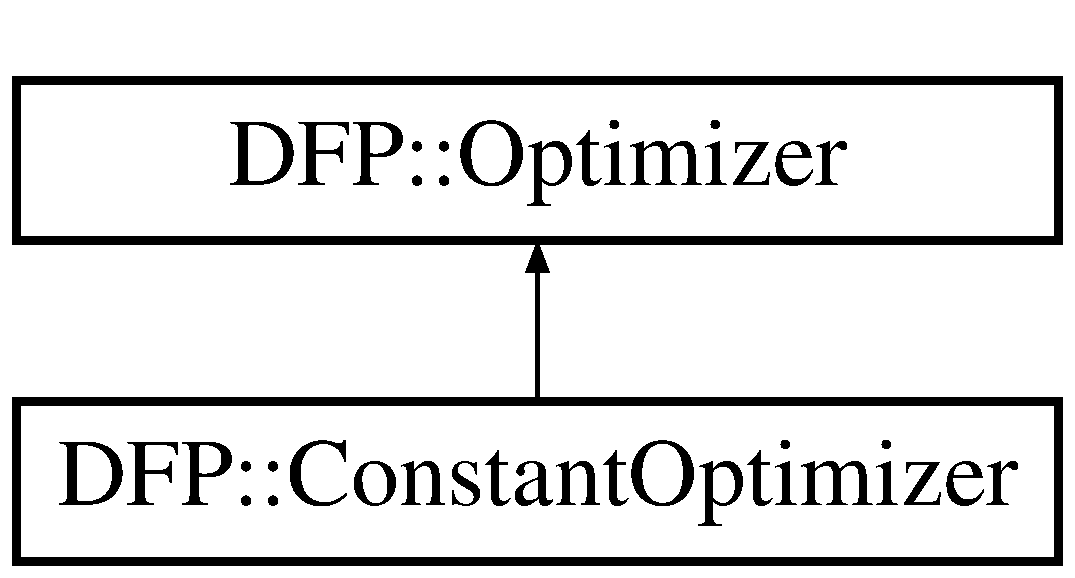
\includegraphics[height=2.000000cm]{class_d_f_p_1_1_constant_optimizer}
\end{center}
\end{figure}
\subsection*{Public Member Functions}
\begin{DoxyCompactItemize}
\item 
\hyperlink{class_d_f_p_1_1_program}{Program} $\ast$ \hyperlink{class_d_f_p_1_1_constant_optimizer_acb6df761c4de78ad622818d400b6f6bd}{optimize} (\hyperlink{class_d_f_p_1_1_program}{Program} $\ast$dfp)\hypertarget{class_d_f_p_1_1_constant_optimizer_acb6df761c4de78ad622818d400b6f6bd}{}\label{class_d_f_p_1_1_constant_optimizer_acb6df761c4de78ad622818d400b6f6bd}

\begin{DoxyCompactList}\small\item\em Virtual function will optimize original \hyperlink{class_d_f_p_1_1_program}{Program} to an optimized \hyperlink{class_d_f_p_1_1_program}{Program}. \end{DoxyCompactList}\end{DoxyCompactItemize}


\subsection{Detailed Description}
Do constant reduction dataflow analysis. 

The documentation for this class was generated from the following files\+:\begin{DoxyCompactItemize}
\item 
include/dfp\+\_\+optimizer.\+hh\item 
src/dfp\+\_\+optimizer.\+cc\end{DoxyCompactItemize}

\hypertarget{class_d_f_p_1_1_edge}{}\section{D\+FP\+:\+:Edge Class Reference}
\label{class_d_f_p_1_1_edge}\index{D\+F\+P\+::\+Edge@{D\+F\+P\+::\+Edge}}


\hyperlink{class_d_f_p_1_1_edge}{Edge} contains pointers to graphs and nodes.  




{\ttfamily \#include $<$dfp\+\_\+program.\+hh$>$}

\subsection*{Public Types}
\begin{DoxyCompactItemize}
\item 
typedef std\+::vector$<$ \hyperlink{class_d_f_p_1_1_edge}{Edge} $\ast$ $>$ \hyperlink{class_d_f_p_1_1_edge_a71ccd1900dbfda5591981064738f60af}{edgelist\+\_\+t}\hypertarget{class_d_f_p_1_1_edge_a71ccd1900dbfda5591981064738f60af}{}\label{class_d_f_p_1_1_edge_a71ccd1900dbfda5591981064738f60af}

\begin{DoxyCompactList}\small\item\em A list contains pointers to \hyperlink{class_d_f_p_1_1_edge}{Edge} objects. \end{DoxyCompactList}\end{DoxyCompactItemize}
\subsection*{Public Member Functions}
\begin{DoxyCompactItemize}
\item 
{\bfseries Edge} (\hyperlink{class_d_f_p_1_1_graph}{Graph} $\ast$g1, \hyperlink{class_d_f_p_1_1_node}{Node} $\ast$n1, \hyperlink{class_d_f_p_1_1_graph}{Graph} $\ast$g2, \hyperlink{class_d_f_p_1_1_node}{Node} $\ast$n2)\hypertarget{class_d_f_p_1_1_edge_a31c5aa0ea975790932d13a18ec6d84ee}{}\label{class_d_f_p_1_1_edge_a31c5aa0ea975790932d13a18ec6d84ee}

\item 
bool {\bfseries validate} ()\hypertarget{class_d_f_p_1_1_edge_a83b1d1a1a421b79d9a181ff4e3e21ecb}{}\label{class_d_f_p_1_1_edge_a83b1d1a1a421b79d9a181ff4e3e21ecb}

\item 
int {\bfseries eval} (int v1, int v2)\hypertarget{class_d_f_p_1_1_edge_ac142939aa6aa05c7ee0713b33af9639e}{}\label{class_d_f_p_1_1_edge_ac142939aa6aa05c7ee0713b33af9639e}

\end{DoxyCompactItemize}
\subsection*{Public Attributes}
\begin{DoxyCompactItemize}
\item 
\hyperlink{class_d_f_p_1_1_graph}{Graph} $\ast$ \hyperlink{class_d_f_p_1_1_edge_a993e651548528b8cc2029d777cf2a881}{src\+\_\+graph}
\item 
\hyperlink{class_d_f_p_1_1_graph}{Graph} $\ast$ \hyperlink{class_d_f_p_1_1_edge_a4f4d043502fb5a3438652bf3fce09273}{dst\+\_\+graph}
\item 
\hyperlink{class_d_f_p_1_1_node}{Node} $\ast$ \hyperlink{class_d_f_p_1_1_edge_a76f03300ad177e767033229d0fc1a780}{src\+\_\+node}
\item 
\hyperlink{class_d_f_p_1_1_node}{Node} $\ast$ \hyperlink{class_d_f_p_1_1_edge_a1c2dd4ca03c0dfa002a2d07dc738cfaa}{dst\+\_\+node}
\end{DoxyCompactItemize}
\subsection*{Friends}
\begin{DoxyCompactItemize}
\item 
std\+::ostream \& {\bfseries operator$<$$<$} (std\+::ostream \&os, const \hyperlink{class_d_f_p_1_1_edge}{Edge} \&e)\hypertarget{class_d_f_p_1_1_edge_aa1b374eb64c6c754621b4fc918a9df57}{}\label{class_d_f_p_1_1_edge_aa1b374eb64c6c754621b4fc918a9df57}

\end{DoxyCompactItemize}


\subsection{Detailed Description}
\hyperlink{class_d_f_p_1_1_edge}{Edge} contains pointers to graphs and nodes. 

\hyperlink{class_d_f_p_1_1_edge}{Edge} contains 4 pointers\+: to the source graph and source node, to the destination graph and node. 

\subsection{Member Data Documentation}
\index{D\+F\+P\+::\+Edge@{D\+F\+P\+::\+Edge}!dst\+\_\+graph@{dst\+\_\+graph}}
\index{dst\+\_\+graph@{dst\+\_\+graph}!D\+F\+P\+::\+Edge@{D\+F\+P\+::\+Edge}}
\subsubsection[{\texorpdfstring{dst\+\_\+graph}{dst_graph}}]{\setlength{\rightskip}{0pt plus 5cm}{\bf Graph}$\ast$ D\+F\+P\+::\+Edge\+::dst\+\_\+graph}\hypertarget{class_d_f_p_1_1_edge_a4f4d043502fb5a3438652bf3fce09273}{}\label{class_d_f_p_1_1_edge_a4f4d043502fb5a3438652bf3fce09273}
Pointers to the desination \hyperlink{class_d_f_p_1_1_graph}{Graph} \index{D\+F\+P\+::\+Edge@{D\+F\+P\+::\+Edge}!dst\+\_\+node@{dst\+\_\+node}}
\index{dst\+\_\+node@{dst\+\_\+node}!D\+F\+P\+::\+Edge@{D\+F\+P\+::\+Edge}}
\subsubsection[{\texorpdfstring{dst\+\_\+node}{dst_node}}]{\setlength{\rightskip}{0pt plus 5cm}{\bf Node}$\ast$ D\+F\+P\+::\+Edge\+::dst\+\_\+node}\hypertarget{class_d_f_p_1_1_edge_a1c2dd4ca03c0dfa002a2d07dc738cfaa}{}\label{class_d_f_p_1_1_edge_a1c2dd4ca03c0dfa002a2d07dc738cfaa}
Pointers to the desination \hyperlink{class_d_f_p_1_1_node}{Node} \index{D\+F\+P\+::\+Edge@{D\+F\+P\+::\+Edge}!src\+\_\+graph@{src\+\_\+graph}}
\index{src\+\_\+graph@{src\+\_\+graph}!D\+F\+P\+::\+Edge@{D\+F\+P\+::\+Edge}}
\subsubsection[{\texorpdfstring{src\+\_\+graph}{src_graph}}]{\setlength{\rightskip}{0pt plus 5cm}{\bf Graph}$\ast$ D\+F\+P\+::\+Edge\+::src\+\_\+graph}\hypertarget{class_d_f_p_1_1_edge_a993e651548528b8cc2029d777cf2a881}{}\label{class_d_f_p_1_1_edge_a993e651548528b8cc2029d777cf2a881}
Pointers to the source \hyperlink{class_d_f_p_1_1_graph}{Graph} \index{D\+F\+P\+::\+Edge@{D\+F\+P\+::\+Edge}!src\+\_\+node@{src\+\_\+node}}
\index{src\+\_\+node@{src\+\_\+node}!D\+F\+P\+::\+Edge@{D\+F\+P\+::\+Edge}}
\subsubsection[{\texorpdfstring{src\+\_\+node}{src_node}}]{\setlength{\rightskip}{0pt plus 5cm}{\bf Node}$\ast$ D\+F\+P\+::\+Edge\+::src\+\_\+node}\hypertarget{class_d_f_p_1_1_edge_a76f03300ad177e767033229d0fc1a780}{}\label{class_d_f_p_1_1_edge_a76f03300ad177e767033229d0fc1a780}
Pointers to the source \hyperlink{class_d_f_p_1_1_node}{Node} 

The documentation for this class was generated from the following files\+:\begin{DoxyCompactItemize}
\item 
include/dfp\+\_\+program.\+hh\item 
src/dfp\+\_\+program.\+cc\end{DoxyCompactItemize}

\hypertarget{class_d_f_p_1_1_graph}{}\section{D\+FP\+:\+:Graph Class Reference}
\label{class_d_f_p_1_1_graph}\index{D\+F\+P\+::\+Graph@{D\+F\+P\+::\+Graph}}


\hyperlink{class_d_f_p_1_1_graph}{Graph} contains a hash table of nodes.  




{\ttfamily \#include $<$dfp\+\_\+program.\+hh$>$}

\subsection*{Public Types}
\begin{DoxyCompactItemize}
\item 
typedef std\+::map$<$ string\+\_\+t, \hyperlink{class_d_f_p_1_1_graph}{Graph} $\ast$ $>$ \hyperlink{class_d_f_p_1_1_graph_ae35638adb932f3b7fd545ac09ea34c5a}{graphtable\+\_\+t}\hypertarget{class_d_f_p_1_1_graph_ae35638adb932f3b7fd545ac09ea34c5a}{}\label{class_d_f_p_1_1_graph_ae35638adb932f3b7fd545ac09ea34c5a}

\begin{DoxyCompactList}\small\item\em A hashtable from graph id to \hyperlink{class_d_f_p_1_1_graph}{Graph} object pointer. \end{DoxyCompactList}\end{DoxyCompactItemize}
\subsection*{Public Member Functions}
\begin{DoxyCompactItemize}
\item 
\hyperlink{class_d_f_p_1_1_graph_a3d04c060d5f07627211996e42e7819fc}{Graph} (string\+\_\+t \hyperlink{class_d_f_p_1_1_graph_aa5ed385b1f994f5220e0bb3d290bcfb8}{id}, \hyperlink{class_d_f_p_1_1_node_a9dc2ef0c0546df091e01cd0df2cc12d9}{Node\+::nodelist\+\_\+t} nl)
\begin{DoxyCompactList}\small\item\em Constructor. \end{DoxyCompactList}\item 
\hyperlink{class_d_f_p_1_1_node_af7bf8e098cd86639fba4160356704786}{Node\+::nodetable\+\_\+t} \hyperlink{class_d_f_p_1_1_graph_a808d6323d5d322df30dcf0703ea5e7fc}{get\+Out\+Node\+Table} ()\hypertarget{class_d_f_p_1_1_graph_a808d6323d5d322df30dcf0703ea5e7fc}{}\label{class_d_f_p_1_1_graph_a808d6323d5d322df30dcf0703ea5e7fc}

\begin{DoxyCompactList}\small\item\em Get the Nodes in this \hyperlink{class_d_f_p_1_1_graph}{Graph} which has type \hyperlink{class_d_f_p_1_1_node_a31d945c7278c3587d6d28c76b0f1ae81ae12934d1eab7d10d4dc8c50c99b765a1}{Node\+::\+Out}. \end{DoxyCompactList}\item 
\hyperlink{class_d_f_p_1_1_node_af7bf8e098cd86639fba4160356704786}{Node\+::nodetable\+\_\+t} \hyperlink{class_d_f_p_1_1_graph_ae045b3ed7d9b2d8da2804d09d34fe46d}{get\+Inp\+Node\+Table} ()\hypertarget{class_d_f_p_1_1_graph_ae045b3ed7d9b2d8da2804d09d34fe46d}{}\label{class_d_f_p_1_1_graph_ae045b3ed7d9b2d8da2804d09d34fe46d}

\begin{DoxyCompactList}\small\item\em Get the Nodes in this \hyperlink{class_d_f_p_1_1_graph}{Graph} which has type \hyperlink{class_d_f_p_1_1_node_a31d945c7278c3587d6d28c76b0f1ae81a8b0ac0a4d07f5860c156947aa7218adc}{Node\+::\+In}. \end{DoxyCompactList}\item 
int \hyperlink{class_d_f_p_1_1_graph_ac39aa15ae1dd24383da300d02b0ae0d1}{get\+Binary\+Node\+Number} ()\hypertarget{class_d_f_p_1_1_graph_ac39aa15ae1dd24383da300d02b0ae0d1}{}\label{class_d_f_p_1_1_graph_ac39aa15ae1dd24383da300d02b0ae0d1}

\begin{DoxyCompactList}\small\item\em Get number of binary nodes. \end{DoxyCompactList}\item 
bool {\bfseries validate} ()\hypertarget{class_d_f_p_1_1_graph_a19063fcb0841ddcd7330129081348e97}{}\label{class_d_f_p_1_1_graph_a19063fcb0841ddcd7330129081348e97}

\end{DoxyCompactItemize}
\subsection*{Public Attributes}
\begin{DoxyCompactItemize}
\item 
string\+\_\+t \hyperlink{class_d_f_p_1_1_graph_aa5ed385b1f994f5220e0bb3d290bcfb8}{id}
\item 
\hyperlink{class_d_f_p_1_1_node_af7bf8e098cd86639fba4160356704786}{Node\+::nodetable\+\_\+t} \hyperlink{class_d_f_p_1_1_graph_a71f3f7d9daf86c8c903f9a0f9428d67d}{nt}
\end{DoxyCompactItemize}
\subsection*{Friends}
\begin{DoxyCompactItemize}
\item 
std\+::ostream \& {\bfseries operator$<$$<$} (std\+::ostream \&os, const \hyperlink{class_d_f_p_1_1_graph}{Graph} \&g)\hypertarget{class_d_f_p_1_1_graph_a63ded41af685d3ec7ab3e6dcac27d7d2}{}\label{class_d_f_p_1_1_graph_a63ded41af685d3ec7ab3e6dcac27d7d2}

\end{DoxyCompactItemize}


\subsection{Detailed Description}
\hyperlink{class_d_f_p_1_1_graph}{Graph} contains a hash table of nodes. 

Each graph contains many Nodes, all the pointers to them will be stored in a hash table, which could be refereced by \hyperlink{class_d_f_p_1_1_node}{Node}\textquotesingle{}s id 

\subsection{Constructor \& Destructor Documentation}
\index{D\+F\+P\+::\+Graph@{D\+F\+P\+::\+Graph}!Graph@{Graph}}
\index{Graph@{Graph}!D\+F\+P\+::\+Graph@{D\+F\+P\+::\+Graph}}
\subsubsection[{\texorpdfstring{Graph(string\+\_\+t id, Node\+::nodelist\+\_\+t nl)}{Graph(string_t id, Node::nodelist_t nl)}}]{\setlength{\rightskip}{0pt plus 5cm}D\+F\+P\+::\+Graph\+::\+Graph (
\begin{DoxyParamCaption}
\item[{string\+\_\+t}]{id, }
\item[{{\bf Node\+::nodelist\+\_\+t}}]{nl}
\end{DoxyParamCaption}
)\hspace{0.3cm}{\ttfamily [inline]}}\hypertarget{class_d_f_p_1_1_graph_a3d04c060d5f07627211996e42e7819fc}{}\label{class_d_f_p_1_1_graph_a3d04c060d5f07627211996e42e7819fc}


Constructor. 

After the parser has parsed the \hyperlink{class_d_f_p_1_1_node}{Node} list within each \hyperlink{class_d_f_p_1_1_graph}{Graph} block, will create a new \hyperlink{class_d_f_p_1_1_graph}{Graph} object by using this collection of \hyperlink{class_d_f_p_1_1_node}{Node}. The original list will be converted to a hash table. 

\subsection{Member Data Documentation}
\index{D\+F\+P\+::\+Graph@{D\+F\+P\+::\+Graph}!id@{id}}
\index{id@{id}!D\+F\+P\+::\+Graph@{D\+F\+P\+::\+Graph}}
\subsubsection[{\texorpdfstring{id}{id}}]{\setlength{\rightskip}{0pt plus 5cm}string\+\_\+t D\+F\+P\+::\+Graph\+::id}\hypertarget{class_d_f_p_1_1_graph_aa5ed385b1f994f5220e0bb3d290bcfb8}{}\label{class_d_f_p_1_1_graph_aa5ed385b1f994f5220e0bb3d290bcfb8}
The id of this \hyperlink{class_d_f_p_1_1_graph}{Graph} \index{D\+F\+P\+::\+Graph@{D\+F\+P\+::\+Graph}!nt@{nt}}
\index{nt@{nt}!D\+F\+P\+::\+Graph@{D\+F\+P\+::\+Graph}}
\subsubsection[{\texorpdfstring{nt}{nt}}]{\setlength{\rightskip}{0pt plus 5cm}{\bf Node\+::nodetable\+\_\+t} D\+F\+P\+::\+Graph\+::nt}\hypertarget{class_d_f_p_1_1_graph_a71f3f7d9daf86c8c903f9a0f9428d67d}{}\label{class_d_f_p_1_1_graph_a71f3f7d9daf86c8c903f9a0f9428d67d}
The hash table in this \hyperlink{class_d_f_p_1_1_graph}{Graph} 

The documentation for this class was generated from the following files\+:\begin{DoxyCompactItemize}
\item 
include/dfp\+\_\+program.\+hh\item 
src/dfp\+\_\+program.\+cc\end{DoxyCompactItemize}

\hypertarget{class_d_f_p_1_1_int_value}{}\section{D\+FP\+:\+:Int\+Value Class Reference}
\label{class_d_f_p_1_1_int_value}\index{D\+F\+P\+::\+Int\+Value@{D\+F\+P\+::\+Int\+Value}}


Inherited from \hyperlink{class_d_f_p_1_1_value}{Value}, to store integer value.  




{\ttfamily \#include $<$dfp\+\_\+program.\+hh$>$}

Inheritance diagram for D\+FP\+:\+:Int\+Value\+:\begin{figure}[H]
\begin{center}
\leavevmode
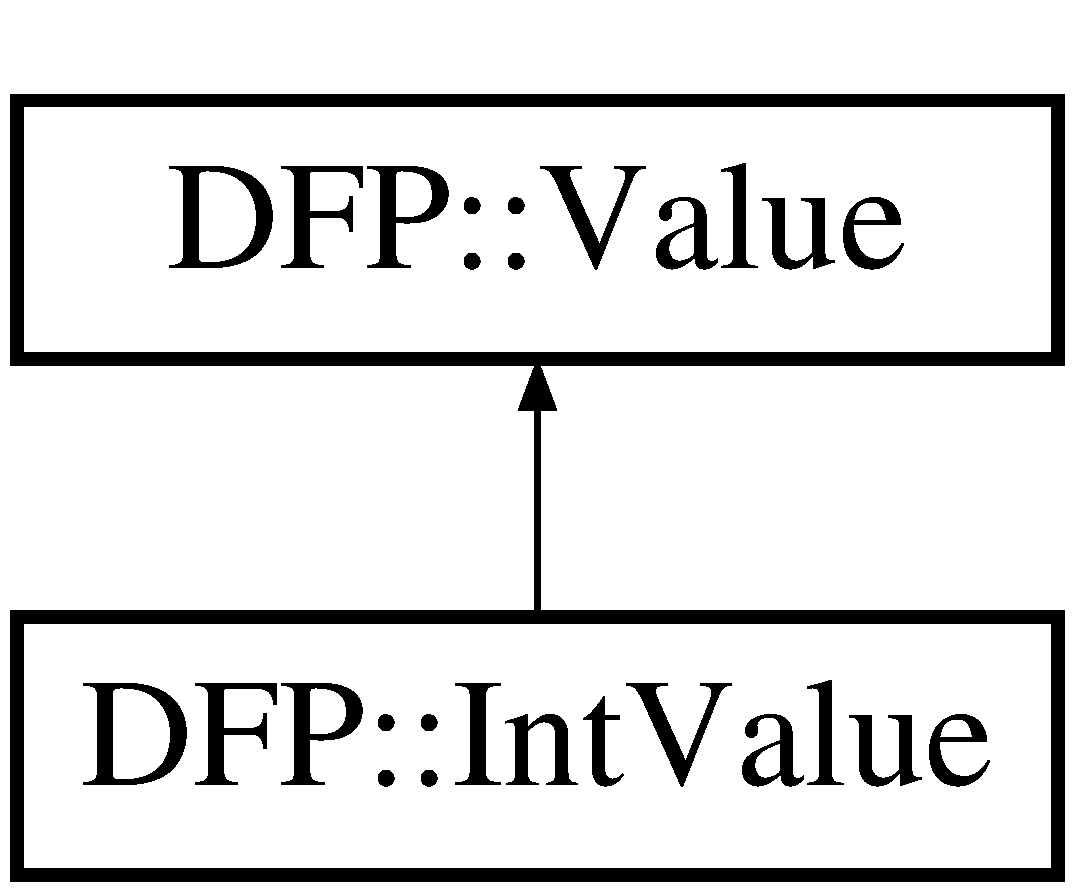
\includegraphics[height=2.000000cm]{class_d_f_p_1_1_int_value}
\end{center}
\end{figure}
\subsection*{Public Member Functions}
\begin{DoxyCompactItemize}
\item 
{\bfseries Int\+Value} (\hyperlink{class_d_f_p_1_1_num}{Num} $\ast$num)\hypertarget{class_d_f_p_1_1_int_value_a088713807e54057ffe84ae332df4d599}{}\label{class_d_f_p_1_1_int_value_a088713807e54057ffe84ae332df4d599}

\end{DoxyCompactItemize}
\subsection*{Static Public Member Functions}
\begin{DoxyCompactItemize}
\item 
static \hyperlink{class_d_f_p_1_1_int_value}{Int\+Value} $\ast$ \hyperlink{class_d_f_p_1_1_int_value_ae48acabd98ba7073ef807f982ebf0964}{create} (int v)\hypertarget{class_d_f_p_1_1_int_value_ae48acabd98ba7073ef807f982ebf0964}{}\label{class_d_f_p_1_1_int_value_ae48acabd98ba7073ef807f982ebf0964}

\begin{DoxyCompactList}\small\item\em Factory method. \end{DoxyCompactList}\end{DoxyCompactItemize}
\subsection*{Public Attributes}
\begin{DoxyCompactItemize}
\item 
int {\bfseries value}\hypertarget{class_d_f_p_1_1_int_value_a8fefd55ca349be95500b1636f5f83144}{}\label{class_d_f_p_1_1_int_value_a8fefd55ca349be95500b1636f5f83144}

\end{DoxyCompactItemize}
\subsection*{Additional Inherited Members}


\subsection{Detailed Description}
Inherited from \hyperlink{class_d_f_p_1_1_value}{Value}, to store integer value. 

The documentation for this class was generated from the following file\+:\begin{DoxyCompactItemize}
\item 
include/dfp\+\_\+program.\+hh\end{DoxyCompactItemize}

\hypertarget{class_d_f_p_1_1_lexer}{}\section{D\+FP\+:\+:Lexer Class Reference}
\label{class_d_f_p_1_1_lexer}\index{D\+F\+P\+::\+Lexer@{D\+F\+P\+::\+Lexer}}
\subsection*{Public Member Functions}
\begin{DoxyCompactItemize}
\item 
{\bfseries Lexer} (F\+I\+LE $\ast$fp)\hypertarget{class_d_f_p_1_1_lexer_a29f761e9983b95cb5c46dfe5c735c77f}{}\label{class_d_f_p_1_1_lexer_a29f761e9983b95cb5c46dfe5c735c77f}

\item 
void {\bfseries reserve} (\hyperlink{class_d_f_p_1_1_word}{Word} $\ast$w)\hypertarget{class_d_f_p_1_1_lexer_aedf6d8e7ced2f9eff243a2ef03667b37}{}\label{class_d_f_p_1_1_lexer_aedf6d8e7ced2f9eff243a2ef03667b37}

\item 
void {\bfseries readch} ()\hypertarget{class_d_f_p_1_1_lexer_ae2318f850f01d5e642a16df7a14bd9e2}{}\label{class_d_f_p_1_1_lexer_ae2318f850f01d5e642a16df7a14bd9e2}

\item 
bool {\bfseries readch} (char c)\hypertarget{class_d_f_p_1_1_lexer_aaa3f0b89cceceb8d78aed1edcd4054cb}{}\label{class_d_f_p_1_1_lexer_aaa3f0b89cceceb8d78aed1edcd4054cb}

\item 
\hyperlink{class_d_f_p_1_1_token}{Token} $\ast$ {\bfseries scan} ()\hypertarget{class_d_f_p_1_1_lexer_ac02a39a39813c137e75f5ea14b5cf937}{}\label{class_d_f_p_1_1_lexer_ac02a39a39813c137e75f5ea14b5cf937}

\end{DoxyCompactItemize}
\subsection*{Static Public Attributes}
\begin{DoxyCompactItemize}
\item 
static int {\bfseries line} = 1\hypertarget{class_d_f_p_1_1_lexer_a44746d995dbbcbd1cf3b1460d9aaf712}{}\label{class_d_f_p_1_1_lexer_a44746d995dbbcbd1cf3b1460d9aaf712}

\end{DoxyCompactItemize}


The documentation for this class was generated from the following files\+:\begin{DoxyCompactItemize}
\item 
include/dfp\+\_\+lexer.\+hh\item 
src/dfp\+\_\+lexer.\+cc\end{DoxyCompactItemize}

\hypertarget{class_d_f_p_1_1_live_var_optimizer}{}\section{D\+FP\+:\+:Live\+Var\+Optimizer Class Reference}
\label{class_d_f_p_1_1_live_var_optimizer}\index{D\+F\+P\+::\+Live\+Var\+Optimizer@{D\+F\+P\+::\+Live\+Var\+Optimizer}}


Do live variables dataflow analysis.  




{\ttfamily \#include $<$dfp\+\_\+optimizer.\+hh$>$}

Inheritance diagram for D\+FP\+:\+:Live\+Var\+Optimizer\+:\begin{figure}[H]
\begin{center}
\leavevmode
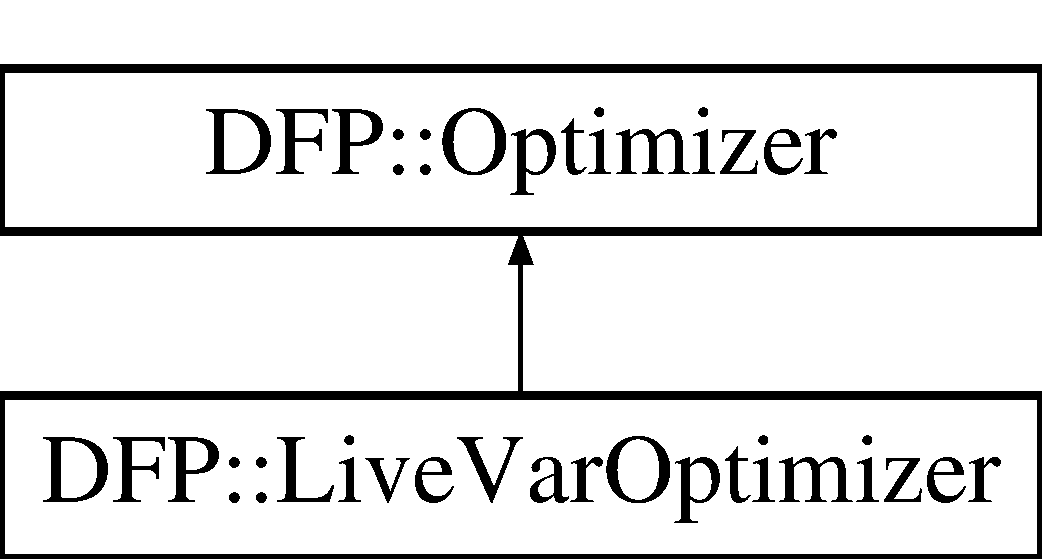
\includegraphics[height=2.000000cm]{class_d_f_p_1_1_live_var_optimizer}
\end{center}
\end{figure}
\subsection*{Public Member Functions}
\begin{DoxyCompactItemize}
\item 
\hyperlink{class_d_f_p_1_1_program}{Program} $\ast$ \hyperlink{class_d_f_p_1_1_live_var_optimizer_a871bc1d15a7f5911a1f040d2baea4ffc}{optimize} (\hyperlink{class_d_f_p_1_1_program}{Program} $\ast$dfp)\hypertarget{class_d_f_p_1_1_live_var_optimizer_a871bc1d15a7f5911a1f040d2baea4ffc}{}\label{class_d_f_p_1_1_live_var_optimizer_a871bc1d15a7f5911a1f040d2baea4ffc}

\begin{DoxyCompactList}\small\item\em Virtual function will optimize original \hyperlink{class_d_f_p_1_1_program}{Program} to an optimized \hyperlink{class_d_f_p_1_1_program}{Program}. \end{DoxyCompactList}\end{DoxyCompactItemize}


\subsection{Detailed Description}
Do live variables dataflow analysis. 

The documentation for this class was generated from the following files\+:\begin{DoxyCompactItemize}
\item 
include/dfp\+\_\+optimizer.\+hh\item 
src/dfp\+\_\+optimizer.\+cc\end{DoxyCompactItemize}

\hypertarget{class_d_f_p_1_1_node}{}\section{D\+FP\+:\+:Node Class Reference}
\label{class_d_f_p_1_1_node}\index{D\+F\+P\+::\+Node@{D\+F\+P\+::\+Node}}


\hyperlink{class_d_f_p_1_1_node}{Node} contains a list of input Values, will be referened in \hyperlink{class_d_f_p_1_1_graph}{Graph} or \hyperlink{class_d_f_p_1_1_edge}{Edge}.  




{\ttfamily \#include $<$dfp\+\_\+program.\+hh$>$}

\subsection*{Public Types}
\begin{DoxyCompactItemize}
\item 
enum \hyperlink{class_d_f_p_1_1_node_a31d945c7278c3587d6d28c76b0f1ae81}{Type} \{ \\*
\hyperlink{class_d_f_p_1_1_node_a31d945c7278c3587d6d28c76b0f1ae81a8b0ac0a4d07f5860c156947aa7218adc}{In}, 
\hyperlink{class_d_f_p_1_1_node_a31d945c7278c3587d6d28c76b0f1ae81ae12934d1eab7d10d4dc8c50c99b765a1}{Out}, 
\hyperlink{class_d_f_p_1_1_node_a31d945c7278c3587d6d28c76b0f1ae81afcb8ac6b8fece66ac56f16db61481373}{Add}, 
\hyperlink{class_d_f_p_1_1_node_a31d945c7278c3587d6d28c76b0f1ae81a428bc0ee7e35107ec42fb0aef0bd65b2}{Sub}, 
\\*
\hyperlink{class_d_f_p_1_1_node_a31d945c7278c3587d6d28c76b0f1ae81a05f8ddf7162817acd31d3ba843e19b07}{Div}, 
\hyperlink{class_d_f_p_1_1_node_a31d945c7278c3587d6d28c76b0f1ae81a4441f6d3c4208c97618533c2bc993b74}{Mult}, 
\hyperlink{class_d_f_p_1_1_node_a31d945c7278c3587d6d28c76b0f1ae81a627eaaffb68dd425c34104e5f8f7d381}{Null}
 \}\begin{DoxyCompactList}\small\item\em An Enum for \hyperlink{class_d_f_p_1_1_node}{Node} object type. \end{DoxyCompactList}
\item 
typedef std\+::map$<$ string\+\_\+t, \hyperlink{class_d_f_p_1_1_node}{Node} $\ast$ $>$ \hyperlink{class_d_f_p_1_1_node_af7bf8e098cd86639fba4160356704786}{nodetable\+\_\+t}\hypertarget{class_d_f_p_1_1_node_af7bf8e098cd86639fba4160356704786}{}\label{class_d_f_p_1_1_node_af7bf8e098cd86639fba4160356704786}

\begin{DoxyCompactList}\small\item\em A hash table from \hyperlink{class_d_f_p_1_1_node}{Node} id string to \hyperlink{class_d_f_p_1_1_node}{Node} object pointer $\ast$/. \end{DoxyCompactList}\item 
typedef std\+::vector$<$ \hyperlink{class_d_f_p_1_1_node}{Node} $\ast$ $>$ \hyperlink{class_d_f_p_1_1_node_a9dc2ef0c0546df091e01cd0df2cc12d9}{nodelist\+\_\+t}\hypertarget{class_d_f_p_1_1_node_a9dc2ef0c0546df091e01cd0df2cc12d9}{}\label{class_d_f_p_1_1_node_a9dc2ef0c0546df091e01cd0df2cc12d9}

\begin{DoxyCompactList}\small\item\em A list of pointers to \hyperlink{class_d_f_p_1_1_node}{Node} objects. \end{DoxyCompactList}\end{DoxyCompactItemize}
\subsection*{Public Member Functions}
\begin{DoxyCompactItemize}
\item 
\hyperlink{class_d_f_p_1_1_node_a41c5c2dfd058d717e46d33e8e2946d91}{Node} (\hyperlink{class_d_f_p_1_1_node_a31d945c7278c3587d6d28c76b0f1ae81}{Type} type, string\+\_\+t \hyperlink{class_d_f_p_1_1_node_a7fb4f15a2c154c960f64797fc887fc75}{id}, \hyperlink{class_d_f_p_1_1_value_a2ca981be3c47c7d23213c08379d3c947}{Value\+::valuelist\+\_\+t} \&\hyperlink{class_d_f_p_1_1_node_aa9e4196de8f357a432508d1bf171a011}{vl})
\begin{DoxyCompactList}\small\item\em Constructor. \end{DoxyCompactList}\item 
bool \hyperlink{class_d_f_p_1_1_node_a61a5b15793ee6f9656c46f4b3f05196a}{is\+Binary} ()
\begin{DoxyCompactList}\small\item\em Check whether this \hyperlink{class_d_f_p_1_1_node}{Node} object is a binary one. \end{DoxyCompactList}\item 
bool \hyperlink{class_d_f_p_1_1_node_afce4058fc5988eb4bf7a33fd519c4d2e}{is\+Unary} ()\hypertarget{class_d_f_p_1_1_node_afce4058fc5988eb4bf7a33fd519c4d2e}{}\label{class_d_f_p_1_1_node_afce4058fc5988eb4bf7a33fd519c4d2e}

\begin{DoxyCompactList}\small\item\em Check whether this \hyperlink{class_d_f_p_1_1_node}{Node} object is a unary one. \end{DoxyCompactList}\item 
int \hyperlink{class_d_f_p_1_1_node_a5abdd9f8ff1d0238fb92f2bf20bd52a1}{eval} (int v1, int v2)\hypertarget{class_d_f_p_1_1_node_a5abdd9f8ff1d0238fb92f2bf20bd52a1}{}\label{class_d_f_p_1_1_node_a5abdd9f8ff1d0238fb92f2bf20bd52a1}

\begin{DoxyCompactList}\small\item\em Use \hyperlink{class_d_f_p_1_1_node}{Node}\textquotesingle{}s type to calculate two input. NO T\+Y\+PE C\+H\+E\+C\+K\+I\+NG H\+E\+R\+E! \end{DoxyCompactList}\end{DoxyCompactItemize}
\subsection*{Static Public Member Functions}
\begin{DoxyCompactItemize}
\item 
static \hyperlink{class_d_f_p_1_1_node_a31d945c7278c3587d6d28c76b0f1ae81}{Type} \hyperlink{class_d_f_p_1_1_node_ac282e4329fb1fcfb791093b40ef4f2aa}{tag2type} (Tag t)\hypertarget{class_d_f_p_1_1_node_ac282e4329fb1fcfb791093b40ef4f2aa}{}\label{class_d_f_p_1_1_node_ac282e4329fb1fcfb791093b40ef4f2aa}

\begin{DoxyCompactList}\small\item\em Convert Tag in \hyperlink{class_d_f_p_1_1_token}{Token} to Type in \hyperlink{class_d_f_p_1_1_node}{Node}. \end{DoxyCompactList}\end{DoxyCompactItemize}
\subsection*{Public Attributes}
\begin{DoxyCompactItemize}
\item 
\hyperlink{class_d_f_p_1_1_node_a31d945c7278c3587d6d28c76b0f1ae81}{Type} {\bfseries type}\hypertarget{class_d_f_p_1_1_node_a51f2b604b13572692ed9579ee7001a8a}{}\label{class_d_f_p_1_1_node_a51f2b604b13572692ed9579ee7001a8a}

\item 
\hyperlink{class_d_f_p_1_1_value_a2ca981be3c47c7d23213c08379d3c947}{Value\+::valuelist\+\_\+t} \hyperlink{class_d_f_p_1_1_node_aa9e4196de8f357a432508d1bf171a011}{vl}
\item 
string\+\_\+t \hyperlink{class_d_f_p_1_1_node_a7fb4f15a2c154c960f64797fc887fc75}{id}
\end{DoxyCompactItemize}
\subsection*{Static Public Attributes}
\begin{DoxyCompactItemize}
\item 
static std\+::string \hyperlink{class_d_f_p_1_1_node_a528f41af98281ae51454cf666d1c04e1}{Type\+Str} \mbox{[}$\,$\mbox{]} = \{\char`\"{}In\char`\"{}, \char`\"{}\hyperlink{class_d_f_p_1_1_node_a31d945c7278c3587d6d28c76b0f1ae81ae12934d1eab7d10d4dc8c50c99b765a1}{Out}\char`\"{}, \char`\"{}\hyperlink{class_d_f_p_1_1_node_a31d945c7278c3587d6d28c76b0f1ae81afcb8ac6b8fece66ac56f16db61481373}{Add}\char`\"{}, \char`\"{}\hyperlink{class_d_f_p_1_1_node_a31d945c7278c3587d6d28c76b0f1ae81a428bc0ee7e35107ec42fb0aef0bd65b2}{Sub}\char`\"{}, \char`\"{}\hyperlink{class_d_f_p_1_1_node_a31d945c7278c3587d6d28c76b0f1ae81a05f8ddf7162817acd31d3ba843e19b07}{Div}\char`\"{}, \char`\"{}\hyperlink{class_d_f_p_1_1_node_a31d945c7278c3587d6d28c76b0f1ae81a4441f6d3c4208c97618533c2bc993b74}{Mult}\char`\"{}, \char`\"{}\hyperlink{class_d_f_p_1_1_node_a31d945c7278c3587d6d28c76b0f1ae81a627eaaffb68dd425c34104e5f8f7d381}{Null}\char`\"{}\}\hypertarget{class_d_f_p_1_1_node_a528f41af98281ae51454cf666d1c04e1}{}\label{class_d_f_p_1_1_node_a528f41af98281ae51454cf666d1c04e1}

\begin{DoxyCompactList}\small\item\em Names for \hyperlink{class_d_f_p_1_1_node_a31d945c7278c3587d6d28c76b0f1ae81}{Node\+::\+Type}. \end{DoxyCompactList}\end{DoxyCompactItemize}
\subsection*{Friends}
\begin{DoxyCompactItemize}
\item 
std\+::ostream \& {\bfseries operator$<$$<$} (std\+::ostream \&os, const \hyperlink{class_d_f_p_1_1_node}{Node} \&n)\hypertarget{class_d_f_p_1_1_node_a6fe565f8d6d1c1d44540c07e92864c91}{}\label{class_d_f_p_1_1_node_a6fe565f8d6d1c1d44540c07e92864c91}

\item 
bool {\bfseries operator==} (const \hyperlink{class_d_f_p_1_1_node}{Node} \&n1, const \hyperlink{class_d_f_p_1_1_node}{Node} \&n2)\hypertarget{class_d_f_p_1_1_node_a156456698e98563a77c4c0af13c20db1}{}\label{class_d_f_p_1_1_node_a156456698e98563a77c4c0af13c20db1}

\end{DoxyCompactItemize}


\subsection{Detailed Description}
\hyperlink{class_d_f_p_1_1_node}{Node} contains a list of input Values, will be referened in \hyperlink{class_d_f_p_1_1_graph}{Graph} or \hyperlink{class_d_f_p_1_1_edge}{Edge}. 

\subsection{Member Enumeration Documentation}
\index{D\+F\+P\+::\+Node@{D\+F\+P\+::\+Node}!Type@{Type}}
\index{Type@{Type}!D\+F\+P\+::\+Node@{D\+F\+P\+::\+Node}}
\subsubsection[{\texorpdfstring{Type}{Type}}]{\setlength{\rightskip}{0pt plus 5cm}enum {\bf D\+F\+P\+::\+Node\+::\+Type}}\hypertarget{class_d_f_p_1_1_node_a31d945c7278c3587d6d28c76b0f1ae81}{}\label{class_d_f_p_1_1_node_a31d945c7278c3587d6d28c76b0f1ae81}


An Enum for \hyperlink{class_d_f_p_1_1_node}{Node} object type. 

Types can be divided into 2 categories\+: Input/\+Output and Binary \begin{Desc}
\item[Enumerator]\par
\begin{description}
\index{In@{In}!D\+F\+P\+::\+Node@{D\+F\+P\+::\+Node}}\index{D\+F\+P\+::\+Node@{D\+F\+P\+::\+Node}!In@{In}}\item[{\em 
In\hypertarget{class_d_f_p_1_1_node_a31d945c7278c3587d6d28c76b0f1ae81a8b0ac0a4d07f5860c156947aa7218adc}{}\label{class_d_f_p_1_1_node_a31d945c7278c3587d6d28c76b0f1ae81a8b0ac0a4d07f5860c156947aa7218adc}
}]This \hyperlink{class_d_f_p_1_1_node}{Node} is an input node, has empty value list. \index{Out@{Out}!D\+F\+P\+::\+Node@{D\+F\+P\+::\+Node}}\index{D\+F\+P\+::\+Node@{D\+F\+P\+::\+Node}!Out@{Out}}\item[{\em 
Out\hypertarget{class_d_f_p_1_1_node_a31d945c7278c3587d6d28c76b0f1ae81ae12934d1eab7d10d4dc8c50c99b765a1}{}\label{class_d_f_p_1_1_node_a31d945c7278c3587d6d28c76b0f1ae81ae12934d1eab7d10d4dc8c50c99b765a1}
}]This \hyperlink{class_d_f_p_1_1_node}{Node} is an output node, has 1 value in the value list \index{Add@{Add}!D\+F\+P\+::\+Node@{D\+F\+P\+::\+Node}}\index{D\+F\+P\+::\+Node@{D\+F\+P\+::\+Node}!Add@{Add}}\item[{\em 
Add\hypertarget{class_d_f_p_1_1_node_a31d945c7278c3587d6d28c76b0f1ae81afcb8ac6b8fece66ac56f16db61481373}{}\label{class_d_f_p_1_1_node_a31d945c7278c3587d6d28c76b0f1ae81afcb8ac6b8fece66ac56f16db61481373}
}]This \hyperlink{class_d_f_p_1_1_node}{Node} will add up two input values \index{Sub@{Sub}!D\+F\+P\+::\+Node@{D\+F\+P\+::\+Node}}\index{D\+F\+P\+::\+Node@{D\+F\+P\+::\+Node}!Sub@{Sub}}\item[{\em 
Sub\hypertarget{class_d_f_p_1_1_node_a31d945c7278c3587d6d28c76b0f1ae81a428bc0ee7e35107ec42fb0aef0bd65b2}{}\label{class_d_f_p_1_1_node_a31d945c7278c3587d6d28c76b0f1ae81a428bc0ee7e35107ec42fb0aef0bd65b2}
}]This \hyperlink{class_d_f_p_1_1_node}{Node} will substract two input values as \mbox{[}0\mbox{]} -\/ \mbox{[}1\mbox{]} \index{Div@{Div}!D\+F\+P\+::\+Node@{D\+F\+P\+::\+Node}}\index{D\+F\+P\+::\+Node@{D\+F\+P\+::\+Node}!Div@{Div}}\item[{\em 
Div\hypertarget{class_d_f_p_1_1_node_a31d945c7278c3587d6d28c76b0f1ae81a05f8ddf7162817acd31d3ba843e19b07}{}\label{class_d_f_p_1_1_node_a31d945c7278c3587d6d28c76b0f1ae81a05f8ddf7162817acd31d3ba843e19b07}
}]This \hyperlink{class_d_f_p_1_1_node}{Node} will multiply two input values \index{Mult@{Mult}!D\+F\+P\+::\+Node@{D\+F\+P\+::\+Node}}\index{D\+F\+P\+::\+Node@{D\+F\+P\+::\+Node}!Mult@{Mult}}\item[{\em 
Mult\hypertarget{class_d_f_p_1_1_node_a31d945c7278c3587d6d28c76b0f1ae81a4441f6d3c4208c97618533c2bc993b74}{}\label{class_d_f_p_1_1_node_a31d945c7278c3587d6d28c76b0f1ae81a4441f6d3c4208c97618533c2bc993b74}
}]This \hyperlink{class_d_f_p_1_1_node}{Node} will divide two input values as \mbox{[}0\mbox{]} / \mbox{[}1\mbox{]} \index{Null@{Null}!D\+F\+P\+::\+Node@{D\+F\+P\+::\+Node}}\index{D\+F\+P\+::\+Node@{D\+F\+P\+::\+Node}!Null@{Null}}\item[{\em 
Null\hypertarget{class_d_f_p_1_1_node_a31d945c7278c3587d6d28c76b0f1ae81a627eaaffb68dd425c34104e5f8f7d381}{}\label{class_d_f_p_1_1_node_a31d945c7278c3587d6d28c76b0f1ae81a627eaaffb68dd425c34104e5f8f7d381}
}]This \hyperlink{class_d_f_p_1_1_node}{Node} can\textquotesingle{}t be recognized \end{description}
\end{Desc}


\subsection{Constructor \& Destructor Documentation}
\index{D\+F\+P\+::\+Node@{D\+F\+P\+::\+Node}!Node@{Node}}
\index{Node@{Node}!D\+F\+P\+::\+Node@{D\+F\+P\+::\+Node}}
\subsubsection[{\texorpdfstring{Node(\+Type type, string\+\_\+t id, Value\+::valuelist\+\_\+t \&vl)}{Node(Type type, string_t id, Value::valuelist_t &vl)}}]{\setlength{\rightskip}{0pt plus 5cm}D\+F\+P\+::\+Node\+::\+Node (
\begin{DoxyParamCaption}
\item[{{\bf Type}}]{type, }
\item[{string\+\_\+t}]{id, }
\item[{{\bf Value\+::valuelist\+\_\+t} \&}]{vl}
\end{DoxyParamCaption}
)\hspace{0.3cm}{\ttfamily [inline]}}\hypertarget{class_d_f_p_1_1_node_a41c5c2dfd058d717e46d33e8e2946d91}{}\label{class_d_f_p_1_1_node_a41c5c2dfd058d717e46d33e8e2946d91}


Constructor. 

Specify the type of the node, the id, and value list for a node. 
\begin{DoxyParams}{Parameters}
{\em type} & The type of this constructing node. \\
\hline
{\em id} & The id for this node. \\
\hline
{\em valuelist} & a list of values parsed before. \\
\hline
\end{DoxyParams}


\subsection{Member Function Documentation}
\index{D\+F\+P\+::\+Node@{D\+F\+P\+::\+Node}!is\+Binary@{is\+Binary}}
\index{is\+Binary@{is\+Binary}!D\+F\+P\+::\+Node@{D\+F\+P\+::\+Node}}
\subsubsection[{\texorpdfstring{is\+Binary()}{isBinary()}}]{\setlength{\rightskip}{0pt plus 5cm}bool D\+F\+P\+::\+Node\+::is\+Binary (
\begin{DoxyParamCaption}
{}
\end{DoxyParamCaption}
)\hspace{0.3cm}{\ttfamily [inline]}}\hypertarget{class_d_f_p_1_1_node_a61a5b15793ee6f9656c46f4b3f05196a}{}\label{class_d_f_p_1_1_node_a61a5b15793ee6f9656c46f4b3f05196a}


Check whether this \hyperlink{class_d_f_p_1_1_node}{Node} object is a binary one. 

The id of this node 

\subsection{Member Data Documentation}
\index{D\+F\+P\+::\+Node@{D\+F\+P\+::\+Node}!id@{id}}
\index{id@{id}!D\+F\+P\+::\+Node@{D\+F\+P\+::\+Node}}
\subsubsection[{\texorpdfstring{id}{id}}]{\setlength{\rightskip}{0pt plus 5cm}string\+\_\+t D\+F\+P\+::\+Node\+::id}\hypertarget{class_d_f_p_1_1_node_a7fb4f15a2c154c960f64797fc887fc75}{}\label{class_d_f_p_1_1_node_a7fb4f15a2c154c960f64797fc887fc75}
The input value list for this \hyperlink{class_d_f_p_1_1_node}{Node} \index{D\+F\+P\+::\+Node@{D\+F\+P\+::\+Node}!vl@{vl}}
\index{vl@{vl}!D\+F\+P\+::\+Node@{D\+F\+P\+::\+Node}}
\subsubsection[{\texorpdfstring{vl}{vl}}]{\setlength{\rightskip}{0pt plus 5cm}{\bf Value\+::valuelist\+\_\+t} D\+F\+P\+::\+Node\+::vl}\hypertarget{class_d_f_p_1_1_node_aa9e4196de8f357a432508d1bf171a011}{}\label{class_d_f_p_1_1_node_aa9e4196de8f357a432508d1bf171a011}
The Type of this \hyperlink{class_d_f_p_1_1_node}{Node} 

The documentation for this class was generated from the following files\+:\begin{DoxyCompactItemize}
\item 
include/dfp\+\_\+program.\+hh\item 
src/dfp\+\_\+program.\+cc\end{DoxyCompactItemize}

\hypertarget{class_d_f_p_1_1_num}{}\section{D\+FP\+:\+:Num Class Reference}
\label{class_d_f_p_1_1_num}\index{D\+F\+P\+::\+Num@{D\+F\+P\+::\+Num}}
Inheritance diagram for D\+FP\+:\+:Num\+:\begin{figure}[H]
\begin{center}
\leavevmode
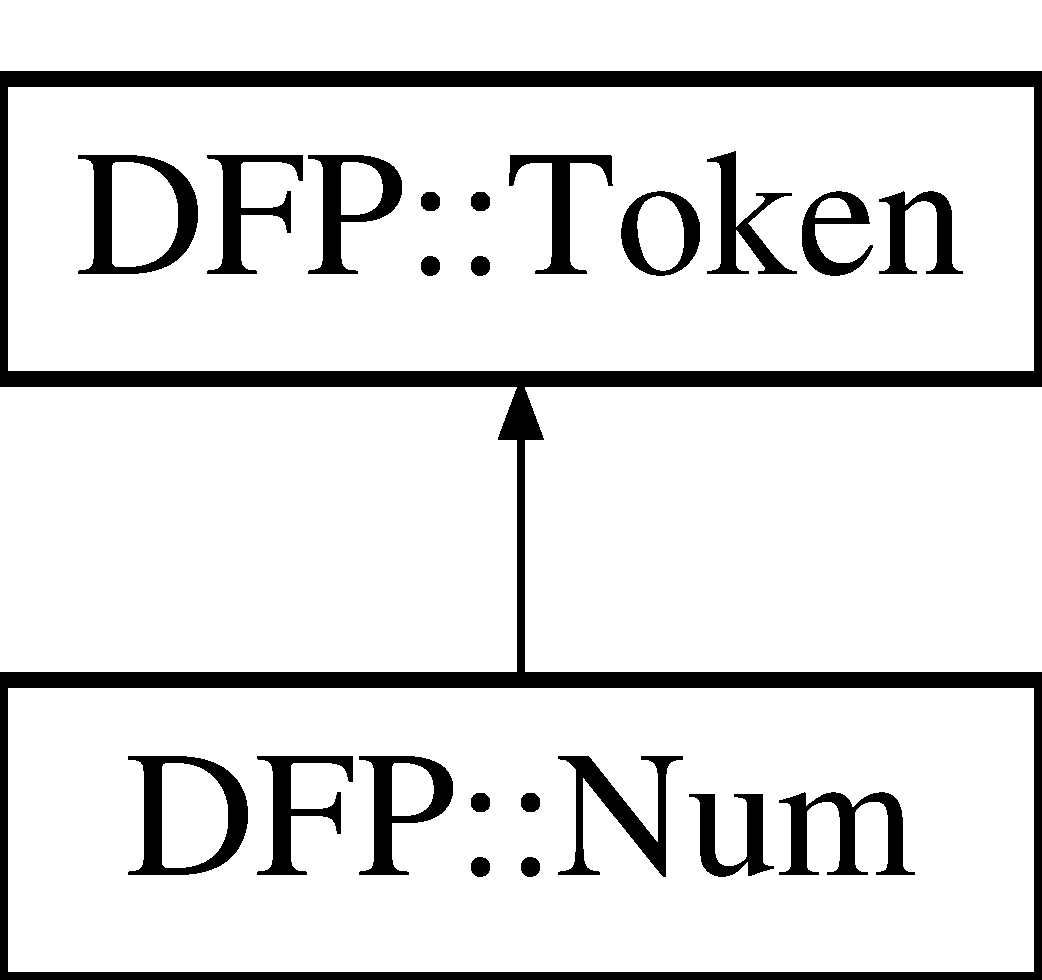
\includegraphics[height=2.000000cm]{class_d_f_p_1_1_num}
\end{center}
\end{figure}
\subsection*{Public Member Functions}
\begin{DoxyCompactItemize}
\item 
{\bfseries Num} (int v)\hypertarget{class_d_f_p_1_1_num_ad35b157c13c9004407103fbc0d66dfc2}{}\label{class_d_f_p_1_1_num_ad35b157c13c9004407103fbc0d66dfc2}

\end{DoxyCompactItemize}
\subsection*{Public Attributes}
\begin{DoxyCompactItemize}
\item 
int {\bfseries value}\hypertarget{class_d_f_p_1_1_num_acd6d8cbedb4d8ca6ab7d71fe6243e90f}{}\label{class_d_f_p_1_1_num_acd6d8cbedb4d8ca6ab7d71fe6243e90f}

\end{DoxyCompactItemize}


The documentation for this class was generated from the following file\+:\begin{DoxyCompactItemize}
\item 
include/dfp\+\_\+lexer.\+hh\end{DoxyCompactItemize}

\hypertarget{class_d_f_p_1_1_optimizer}{}\section{D\+FP\+:\+:Optimizer Class Reference}
\label{class_d_f_p_1_1_optimizer}\index{D\+F\+P\+::\+Optimizer@{D\+F\+P\+::\+Optimizer}}


Base optimizer class for different optimize methods.  




{\ttfamily \#include $<$dfp\+\_\+optimizer.\+hh$>$}

Inheritance diagram for D\+FP\+:\+:Optimizer\+:\begin{figure}[H]
\begin{center}
\leavevmode
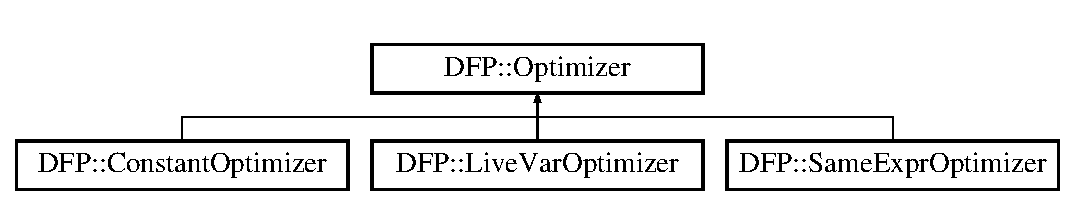
\includegraphics[height=2.000000cm]{class_d_f_p_1_1_optimizer}
\end{center}
\end{figure}
\subsection*{Public Member Functions}
\begin{DoxyCompactItemize}
\item 
virtual \hyperlink{class_d_f_p_1_1_program}{Program} $\ast$ \hyperlink{class_d_f_p_1_1_optimizer_a192e408971c647a028e7c6a2282adc43}{optimize} (\hyperlink{class_d_f_p_1_1_program}{Program} $\ast$dfp)\hypertarget{class_d_f_p_1_1_optimizer_a192e408971c647a028e7c6a2282adc43}{}\label{class_d_f_p_1_1_optimizer_a192e408971c647a028e7c6a2282adc43}

\begin{DoxyCompactList}\small\item\em Virtual function will optimize original \hyperlink{class_d_f_p_1_1_program}{Program} to an optimized \hyperlink{class_d_f_p_1_1_program}{Program}. \end{DoxyCompactList}\end{DoxyCompactItemize}


\subsection{Detailed Description}
Base optimizer class for different optimize methods. 

The documentation for this class was generated from the following file\+:\begin{DoxyCompactItemize}
\item 
include/dfp\+\_\+optimizer.\+hh\end{DoxyCompactItemize}

\hypertarget{class_d_f_p_1_1_parser}{}\section{D\+FP\+:\+:Parser Class Reference}
\label{class_d_f_p_1_1_parser}\index{D\+F\+P\+::\+Parser@{D\+F\+P\+::\+Parser}}
\subsection*{Public Member Functions}
\begin{DoxyCompactItemize}
\item 
{\bfseries Parser} (\hyperlink{class_d_f_p_1_1_lexer}{Lexer} $\ast$l)\hypertarget{class_d_f_p_1_1_parser_a7f48d3c0a6dcb12cf40a95ebd36c1627}{}\label{class_d_f_p_1_1_parser_a7f48d3c0a6dcb12cf40a95ebd36c1627}

\item 
void {\bfseries move} ()\hypertarget{class_d_f_p_1_1_parser_a4ba579f89d51d234369980b746a74d93}{}\label{class_d_f_p_1_1_parser_a4ba579f89d51d234369980b746a74d93}

\item 
void {\bfseries match} (int t)\hypertarget{class_d_f_p_1_1_parser_a78f9e18b8de4c3590beae7ea04037651}{}\label{class_d_f_p_1_1_parser_a78f9e18b8de4c3590beae7ea04037651}

\item 
\hyperlink{class_d_f_p_1_1_program}{Program} $\ast$ {\bfseries program} ()\hypertarget{class_d_f_p_1_1_parser_a90bfc769259c19c87b38621873979caf}{}\label{class_d_f_p_1_1_parser_a90bfc769259c19c87b38621873979caf}

\item 
\hyperlink{class_d_f_p_1_1_graph}{Graph} $\ast$ {\bfseries graph} ()\hypertarget{class_d_f_p_1_1_parser_a952e9d99f203e4ed0b0bcddf881bcab4}{}\label{class_d_f_p_1_1_parser_a952e9d99f203e4ed0b0bcddf881bcab4}

\item 
\hyperlink{class_d_f_p_1_1_node}{Node} $\ast$ {\bfseries node} ()\hypertarget{class_d_f_p_1_1_parser_af1d347b564b46208d41d6867d138da27}{}\label{class_d_f_p_1_1_parser_af1d347b564b46208d41d6867d138da27}

\item 
\hyperlink{class_d_f_p_1_1_node_a9dc2ef0c0546df091e01cd0df2cc12d9}{Node\+::nodelist\+\_\+t} {\bfseries nodelist} ()\hypertarget{class_d_f_p_1_1_parser_aa19cce628b0caf2492b43b5443c308d6}{}\label{class_d_f_p_1_1_parser_aa19cce628b0caf2492b43b5443c308d6}

\item 
\hyperlink{class_d_f_p_1_1_value}{Value} $\ast$ {\bfseries value} ()\hypertarget{class_d_f_p_1_1_parser_ab2ab2eccceabc1400575f0340269fd6a}{}\label{class_d_f_p_1_1_parser_ab2ab2eccceabc1400575f0340269fd6a}

\item 
\hyperlink{class_d_f_p_1_1_value_a2ca981be3c47c7d23213c08379d3c947}{Value\+::valuelist\+\_\+t} {\bfseries valuelist} ()\hypertarget{class_d_f_p_1_1_parser_af5c91f86af0f7e1d5d2440ee5fbf9a5e}{}\label{class_d_f_p_1_1_parser_af5c91f86af0f7e1d5d2440ee5fbf9a5e}

\item 
\hyperlink{class_d_f_p_1_1_edge}{Edge} $\ast$ {\bfseries edge} ()\hypertarget{class_d_f_p_1_1_parser_a5f5041ecadedaf2aa149d78fdd104735}{}\label{class_d_f_p_1_1_parser_a5f5041ecadedaf2aa149d78fdd104735}

\end{DoxyCompactItemize}
\subsection*{Public Attributes}
\begin{DoxyCompactItemize}
\item 
\hyperlink{class_d_f_p_1_1_graph_ae35638adb932f3b7fd545ac09ea34c5a}{Graph\+::graphtable\+\_\+t} {\bfseries graphs}\hypertarget{class_d_f_p_1_1_parser_af97bf674f2c2460b71131afa38437e7f}{}\label{class_d_f_p_1_1_parser_af97bf674f2c2460b71131afa38437e7f}

\item 
\hyperlink{class_d_f_p_1_1_edge_a71ccd1900dbfda5591981064738f60af}{Edge\+::edgelist\+\_\+t} {\bfseries edges}\hypertarget{class_d_f_p_1_1_parser_a3de52a397448d3de34d4ef5c84798f3a}{}\label{class_d_f_p_1_1_parser_a3de52a397448d3de34d4ef5c84798f3a}

\end{DoxyCompactItemize}


The documentation for this class was generated from the following files\+:\begin{DoxyCompactItemize}
\item 
include/dfp\+\_\+parser.\+hh\item 
src/dfp\+\_\+parser.\+cc\end{DoxyCompactItemize}

\hypertarget{class_d_f_p_1_1_program}{}\section{D\+FP\+:\+:Program Class Reference}
\label{class_d_f_p_1_1_program}\index{D\+F\+P\+::\+Program@{D\+F\+P\+::\+Program}}


\hyperlink{class_d_f_p_1_1_program}{Program} contains references to Graphs and Nodes.  




{\ttfamily \#include $<$dfp\+\_\+program.\+hh$>$}

\subsection*{Public Types}
\begin{DoxyCompactItemize}
\item 
typedef std\+::map$<$ string\+\_\+t, int $>$ {\bfseries report\+\_\+t}\hypertarget{class_d_f_p_1_1_program_aeaaa020ec93ac51b61399ba349e6ca64}{}\label{class_d_f_p_1_1_program_aeaaa020ec93ac51b61399ba349e6ca64}

\end{DoxyCompactItemize}
\subsection*{Public Member Functions}
\begin{DoxyCompactItemize}
\item 
{\bfseries Program} (\hyperlink{class_d_f_p_1_1_graph_ae35638adb932f3b7fd545ac09ea34c5a}{Graph\+::graphtable\+\_\+t} \&gs, \hyperlink{class_d_f_p_1_1_edge_a71ccd1900dbfda5591981064738f60af}{Edge\+::edgelist\+\_\+t} \&es)\hypertarget{class_d_f_p_1_1_program_a08995326789c0e0fdea41d36fc90584c}{}\label{class_d_f_p_1_1_program_a08995326789c0e0fdea41d36fc90584c}

\item 
report\+\_\+t \hyperlink{class_d_f_p_1_1_program_a0e2b0b5a6fd02902742c1728679872e9}{get\+Report} ()\hypertarget{class_d_f_p_1_1_program_a0e2b0b5a6fd02902742c1728679872e9}{}\label{class_d_f_p_1_1_program_a0e2b0b5a6fd02902742c1728679872e9}

\begin{DoxyCompactList}\small\item\em Get total number of binary nodes in all graphs. \end{DoxyCompactList}\end{DoxyCompactItemize}
\subsection*{Public Attributes}
\begin{DoxyCompactItemize}
\item 
\hyperlink{class_d_f_p_1_1_graph_ae35638adb932f3b7fd545ac09ea34c5a}{Graph\+::graphtable\+\_\+t} {\bfseries graphs}\hypertarget{class_d_f_p_1_1_program_a2a5742b3d9dfa492901729b919c22abc}{}\label{class_d_f_p_1_1_program_a2a5742b3d9dfa492901729b919c22abc}

\item 
\hyperlink{class_d_f_p_1_1_edge_a71ccd1900dbfda5591981064738f60af}{Edge\+::edgelist\+\_\+t} {\bfseries edges}\hypertarget{class_d_f_p_1_1_program_a4356cd8b3396652e8fde0104d980f176}{}\label{class_d_f_p_1_1_program_a4356cd8b3396652e8fde0104d980f176}

\end{DoxyCompactItemize}
\subsection*{Friends}
\begin{DoxyCompactItemize}
\item 
std\+::ostream \& {\bfseries operator$<$$<$} (std\+::ostream \&os, const \hyperlink{class_d_f_p_1_1_program}{Program} \&dfg)\hypertarget{class_d_f_p_1_1_program_a72cc270a3f767cf145203704dfe87d11}{}\label{class_d_f_p_1_1_program_a72cc270a3f767cf145203704dfe87d11}

\end{DoxyCompactItemize}


\subsection{Detailed Description}
\hyperlink{class_d_f_p_1_1_program}{Program} contains references to Graphs and Nodes. 

Each \hyperlink{class_d_f_p_1_1_program}{Program} has a hash table of Graphs and a list of Nodes. It\textquotesingle{}s the main object we need to handle with after the parser. 

The documentation for this class was generated from the following files\+:\begin{DoxyCompactItemize}
\item 
include/dfp\+\_\+program.\+hh\item 
src/dfp\+\_\+program.\+cc\end{DoxyCompactItemize}

\hypertarget{class_d_f_p_1_1_same_expr_optimizer}{}\section{D\+FP\+:\+:Same\+Expr\+Optimizer Class Reference}
\label{class_d_f_p_1_1_same_expr_optimizer}\index{D\+F\+P\+::\+Same\+Expr\+Optimizer@{D\+F\+P\+::\+Same\+Expr\+Optimizer}}


Do same expression reduction dataflow analysis.  




{\ttfamily \#include $<$dfp\+\_\+optimizer.\+hh$>$}

Inheritance diagram for D\+FP\+:\+:Same\+Expr\+Optimizer\+:\begin{figure}[H]
\begin{center}
\leavevmode
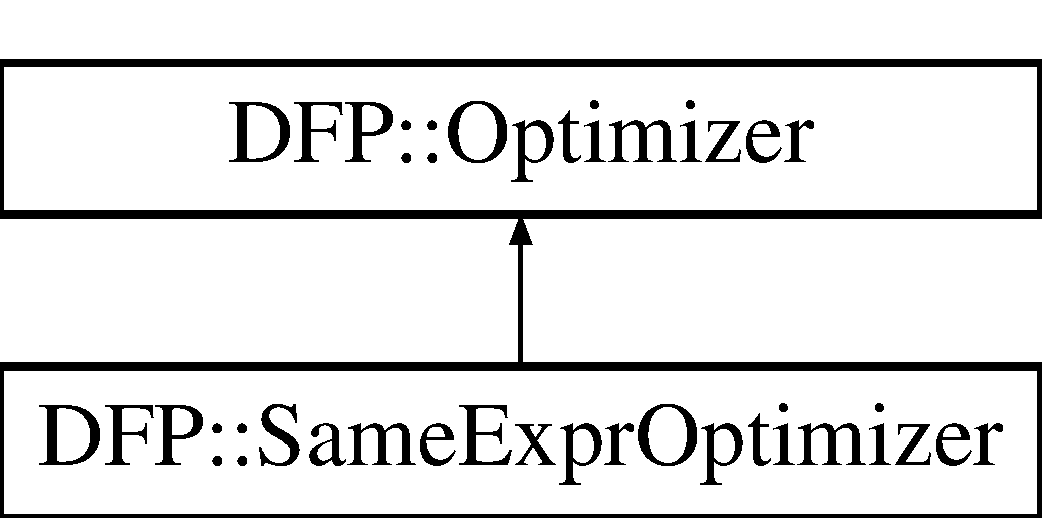
\includegraphics[height=2.000000cm]{class_d_f_p_1_1_same_expr_optimizer}
\end{center}
\end{figure}
\subsection*{Public Member Functions}
\begin{DoxyCompactItemize}
\item 
\hyperlink{class_d_f_p_1_1_program}{Program} $\ast$ \hyperlink{class_d_f_p_1_1_same_expr_optimizer_acf0209f121e89ba066c8d9020fcba0da}{optimize} (\hyperlink{class_d_f_p_1_1_program}{Program} $\ast$dfp)\hypertarget{class_d_f_p_1_1_same_expr_optimizer_acf0209f121e89ba066c8d9020fcba0da}{}\label{class_d_f_p_1_1_same_expr_optimizer_acf0209f121e89ba066c8d9020fcba0da}

\begin{DoxyCompactList}\small\item\em Virtual function will optimize original \hyperlink{class_d_f_p_1_1_program}{Program} to an optimized \hyperlink{class_d_f_p_1_1_program}{Program}. \end{DoxyCompactList}\end{DoxyCompactItemize}


\subsection{Detailed Description}
Do same expression reduction dataflow analysis. 

The documentation for this class was generated from the following files\+:\begin{DoxyCompactItemize}
\item 
include/dfp\+\_\+optimizer.\+hh\item 
src/dfp\+\_\+optimizer.\+cc\end{DoxyCompactItemize}

\hypertarget{class_d_f_p_1_1_str_value}{}\section{D\+FP\+:\+:Str\+Value Class Reference}
\label{class_d_f_p_1_1_str_value}\index{D\+F\+P\+::\+Str\+Value@{D\+F\+P\+::\+Str\+Value}}


Inherited from \hyperlink{class_d_f_p_1_1_value}{Value}, to store string value.  




{\ttfamily \#include $<$dfp\+\_\+program.\+hh$>$}

Inheritance diagram for D\+FP\+:\+:Str\+Value\+:\begin{figure}[H]
\begin{center}
\leavevmode
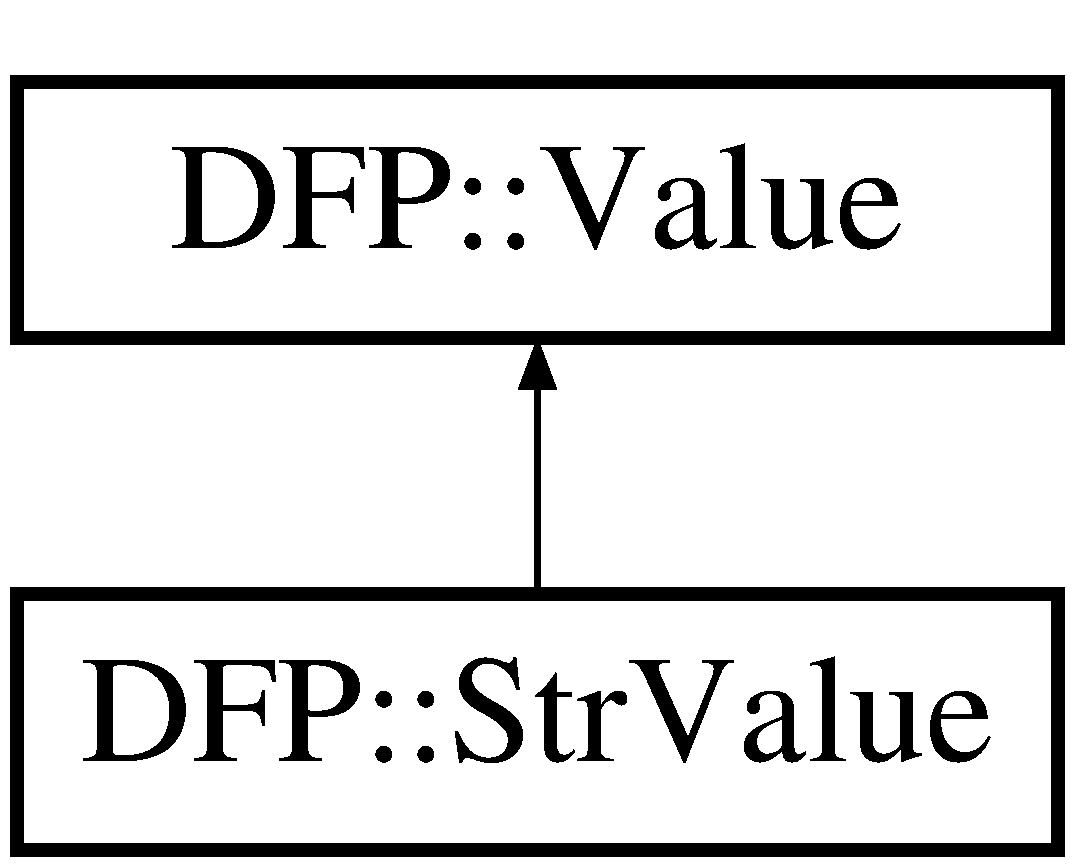
\includegraphics[height=2.000000cm]{class_d_f_p_1_1_str_value}
\end{center}
\end{figure}
\subsection*{Public Member Functions}
\begin{DoxyCompactItemize}
\item 
{\bfseries Str\+Value} (\hyperlink{class_d_f_p_1_1_word}{Word} $\ast$word)\hypertarget{class_d_f_p_1_1_str_value_a8a7c872f531c50246a0095e4df8f11a7}{}\label{class_d_f_p_1_1_str_value_a8a7c872f531c50246a0095e4df8f11a7}

\end{DoxyCompactItemize}
\subsection*{Static Public Member Functions}
\begin{DoxyCompactItemize}
\item 
static \hyperlink{class_d_f_p_1_1_str_value}{Str\+Value} $\ast$ \hyperlink{class_d_f_p_1_1_str_value_a7870713b8d1748f6f460412a5420a85e}{create} (string\+\_\+t s)\hypertarget{class_d_f_p_1_1_str_value_a7870713b8d1748f6f460412a5420a85e}{}\label{class_d_f_p_1_1_str_value_a7870713b8d1748f6f460412a5420a85e}

\begin{DoxyCompactList}\small\item\em Factory method. \end{DoxyCompactList}\end{DoxyCompactItemize}
\subsection*{Public Attributes}
\begin{DoxyCompactItemize}
\item 
string\+\_\+t {\bfseries value}\hypertarget{class_d_f_p_1_1_str_value_aa73f37af1d825788bfbc10cf74276876}{}\label{class_d_f_p_1_1_str_value_aa73f37af1d825788bfbc10cf74276876}

\end{DoxyCompactItemize}
\subsection*{Additional Inherited Members}


\subsection{Detailed Description}
Inherited from \hyperlink{class_d_f_p_1_1_value}{Value}, to store string value. 

The documentation for this class was generated from the following file\+:\begin{DoxyCompactItemize}
\item 
include/dfp\+\_\+program.\+hh\end{DoxyCompactItemize}

\hypertarget{class_d_f_p_1_1_token}{}\section{D\+FP\+:\+:Token Class Reference}
\label{class_d_f_p_1_1_token}\index{D\+F\+P\+::\+Token@{D\+F\+P\+::\+Token}}
Inheritance diagram for D\+FP\+:\+:Token\+:\begin{figure}[H]
\begin{center}
\leavevmode
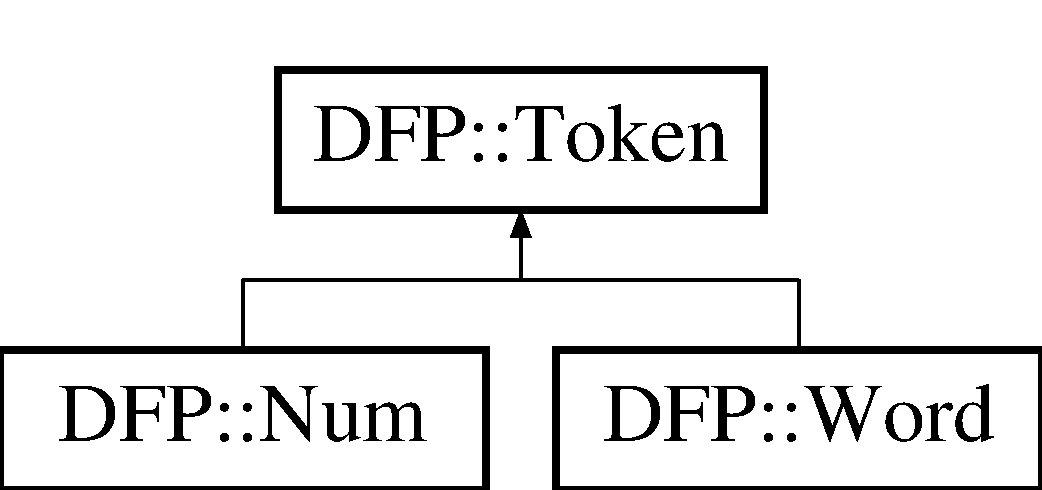
\includegraphics[height=2.000000cm]{class_d_f_p_1_1_token}
\end{center}
\end{figure}
\subsection*{Public Member Functions}
\begin{DoxyCompactItemize}
\item 
{\bfseries Token} (int t)\hypertarget{class_d_f_p_1_1_token_a6ce43ce39be66b0d78cf3160f4f6c448}{}\label{class_d_f_p_1_1_token_a6ce43ce39be66b0d78cf3160f4f6c448}

\end{DoxyCompactItemize}
\subsection*{Public Attributes}
\begin{DoxyCompactItemize}
\item 
int {\bfseries tag}\hypertarget{class_d_f_p_1_1_token_a696bd129a31cf17f47df4e4ebae80fe0}{}\label{class_d_f_p_1_1_token_a696bd129a31cf17f47df4e4ebae80fe0}

\end{DoxyCompactItemize}


The documentation for this class was generated from the following file\+:\begin{DoxyCompactItemize}
\item 
include/dfp\+\_\+lexer.\+hh\end{DoxyCompactItemize}

\hypertarget{class_d_f_p_1_1_value}{}\section{D\+FP\+:\+:Value Class Reference}
\label{class_d_f_p_1_1_value}\index{D\+F\+P\+::\+Value@{D\+F\+P\+::\+Value}}


\hyperlink{class_d_f_p_1_1_value}{Value} stores the elements in each \hyperlink{class_d_f_p_1_1_node}{Node}\textquotesingle{}s input list.  




{\ttfamily \#include $<$dfp\+\_\+program.\+hh$>$}

Inheritance diagram for D\+FP\+:\+:Value\+:\begin{figure}[H]
\begin{center}
\leavevmode
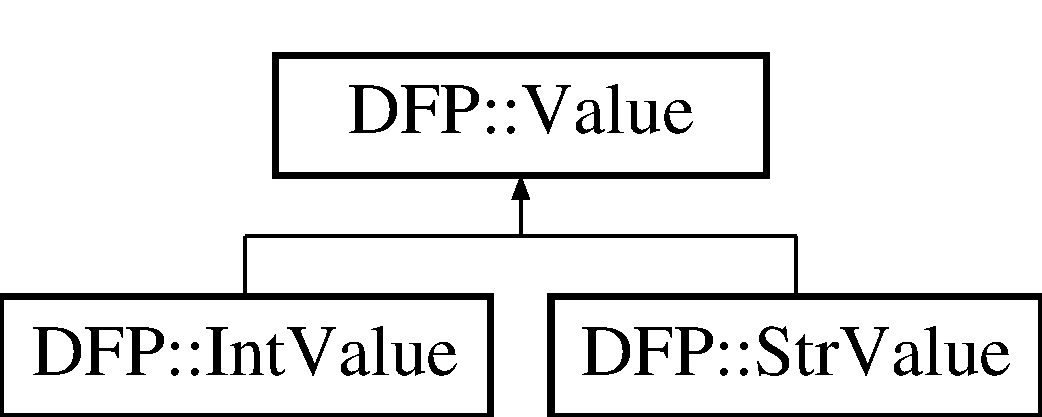
\includegraphics[height=2.000000cm]{class_d_f_p_1_1_value}
\end{center}
\end{figure}
\subsection*{Public Types}
\begin{DoxyCompactItemize}
\item 
enum \hyperlink{class_d_f_p_1_1_value_ab50504401cc3c884a5c6eb8708f8a214}{Type} \{ \hyperlink{class_d_f_p_1_1_value_ab50504401cc3c884a5c6eb8708f8a214a0a8aa2cb5add38d33229c160220a5456}{Int\+Type}, 
\hyperlink{class_d_f_p_1_1_value_ab50504401cc3c884a5c6eb8708f8a214a07b832a0a41fd9d2402d688010a733d6}{Str\+Type}
 \}\begin{DoxyCompactList}\small\item\em An Enum for \hyperlink{class_d_f_p_1_1_value}{Value} object type. \end{DoxyCompactList}
\item 
typedef std\+::vector$<$ \hyperlink{class_d_f_p_1_1_value}{Value} $\ast$ $>$ \hyperlink{class_d_f_p_1_1_value_a2ca981be3c47c7d23213c08379d3c947}{valuelist\+\_\+t}\hypertarget{class_d_f_p_1_1_value_a2ca981be3c47c7d23213c08379d3c947}{}\label{class_d_f_p_1_1_value_a2ca981be3c47c7d23213c08379d3c947}

\begin{DoxyCompactList}\small\item\em A list of pointers to \hyperlink{class_d_f_p_1_1_value}{Value} objects. \end{DoxyCompactList}\end{DoxyCompactItemize}
\subsection*{Public Member Functions}
\begin{DoxyCompactItemize}
\item 
\hyperlink{class_d_f_p_1_1_value_ab4bc39c8d0e04a5adf709e9b339ae930}{Value} (\hyperlink{class_d_f_p_1_1_token}{Token} $\ast$\hyperlink{class_d_f_p_1_1_value_a4cfafb890922feafab6d842a85812d10}{token}, \hyperlink{class_d_f_p_1_1_value_ab50504401cc3c884a5c6eb8708f8a214}{Type} \hyperlink{class_d_f_p_1_1_value_ae2c49913c035b9400361438ef5fe0f8e}{type})
\begin{DoxyCompactList}\small\item\em Constructor. \end{DoxyCompactList}\end{DoxyCompactItemize}
\subsection*{Public Attributes}
\begin{DoxyCompactItemize}
\item 
\hyperlink{class_d_f_p_1_1_token}{Token} $\ast$ \hyperlink{class_d_f_p_1_1_value_a4cfafb890922feafab6d842a85812d10}{token}
\item 
\hyperlink{class_d_f_p_1_1_value_ab50504401cc3c884a5c6eb8708f8a214}{Type} \hyperlink{class_d_f_p_1_1_value_ae2c49913c035b9400361438ef5fe0f8e}{type}
\end{DoxyCompactItemize}
\subsection*{Friends}
\begin{DoxyCompactItemize}
\item 
std\+::ostream \& {\bfseries operator$<$$<$} (std\+::ostream \&os, const \hyperlink{class_d_f_p_1_1_value}{Value} \&v)\hypertarget{class_d_f_p_1_1_value_ad29db86c4a2dec5bc8d0006031b07211}{}\label{class_d_f_p_1_1_value_ad29db86c4a2dec5bc8d0006031b07211}

\item 
bool {\bfseries operator==} (const \hyperlink{class_d_f_p_1_1_value}{Value} \&v1, const \hyperlink{class_d_f_p_1_1_value}{Value} \&v2)\hypertarget{class_d_f_p_1_1_value_afd4eae14a112344d5be0a51bd913941c}{}\label{class_d_f_p_1_1_value_afd4eae14a112344d5be0a51bd913941c}

\end{DoxyCompactItemize}


\subsection{Detailed Description}
\hyperlink{class_d_f_p_1_1_value}{Value} stores the elements in each \hyperlink{class_d_f_p_1_1_node}{Node}\textquotesingle{}s input list. 

This class has design defects, it should be better with templates 

\subsection{Member Enumeration Documentation}
\index{D\+F\+P\+::\+Value@{D\+F\+P\+::\+Value}!Type@{Type}}
\index{Type@{Type}!D\+F\+P\+::\+Value@{D\+F\+P\+::\+Value}}
\subsubsection[{\texorpdfstring{Type}{Type}}]{\setlength{\rightskip}{0pt plus 5cm}enum {\bf D\+F\+P\+::\+Value\+::\+Type}}\hypertarget{class_d_f_p_1_1_value_ab50504401cc3c884a5c6eb8708f8a214}{}\label{class_d_f_p_1_1_value_ab50504401cc3c884a5c6eb8708f8a214}


An Enum for \hyperlink{class_d_f_p_1_1_value}{Value} object type. 

\begin{Desc}
\item[Enumerator]\par
\begin{description}
\index{Int\+Type@{Int\+Type}!D\+F\+P\+::\+Value@{D\+F\+P\+::\+Value}}\index{D\+F\+P\+::\+Value@{D\+F\+P\+::\+Value}!Int\+Type@{Int\+Type}}\item[{\em 
Int\+Type\hypertarget{class_d_f_p_1_1_value_ab50504401cc3c884a5c6eb8708f8a214a0a8aa2cb5add38d33229c160220a5456}{}\label{class_d_f_p_1_1_value_ab50504401cc3c884a5c6eb8708f8a214a0a8aa2cb5add38d33229c160220a5456}
}]This value is an integer \index{Str\+Type@{Str\+Type}!D\+F\+P\+::\+Value@{D\+F\+P\+::\+Value}}\index{D\+F\+P\+::\+Value@{D\+F\+P\+::\+Value}!Str\+Type@{Str\+Type}}\item[{\em 
Str\+Type\hypertarget{class_d_f_p_1_1_value_ab50504401cc3c884a5c6eb8708f8a214a07b832a0a41fd9d2402d688010a733d6}{}\label{class_d_f_p_1_1_value_ab50504401cc3c884a5c6eb8708f8a214a07b832a0a41fd9d2402d688010a733d6}
}]This value is a string \end{description}
\end{Desc}


\subsection{Constructor \& Destructor Documentation}
\index{D\+F\+P\+::\+Value@{D\+F\+P\+::\+Value}!Value@{Value}}
\index{Value@{Value}!D\+F\+P\+::\+Value@{D\+F\+P\+::\+Value}}
\subsubsection[{\texorpdfstring{Value(\+Token $\ast$token, Type type)}{Value(Token *token, Type type)}}]{\setlength{\rightskip}{0pt plus 5cm}D\+F\+P\+::\+Value\+::\+Value (
\begin{DoxyParamCaption}
\item[{{\bf Token} $\ast$}]{token, }
\item[{{\bf Type}}]{type}
\end{DoxyParamCaption}
)\hspace{0.3cm}{\ttfamily [inline]}}\hypertarget{class_d_f_p_1_1_value_ab4bc39c8d0e04a5adf709e9b339ae930}{}\label{class_d_f_p_1_1_value_ab4bc39c8d0e04a5adf709e9b339ae930}


Constructor. 

Takes a token and assign the type 

\subsection{Member Data Documentation}
\index{D\+F\+P\+::\+Value@{D\+F\+P\+::\+Value}!token@{token}}
\index{token@{token}!D\+F\+P\+::\+Value@{D\+F\+P\+::\+Value}}
\subsubsection[{\texorpdfstring{token}{token}}]{\setlength{\rightskip}{0pt plus 5cm}{\bf Token}$\ast$ D\+F\+P\+::\+Value\+::token}\hypertarget{class_d_f_p_1_1_value_a4cfafb890922feafab6d842a85812d10}{}\label{class_d_f_p_1_1_value_a4cfafb890922feafab6d842a85812d10}
\hyperlink{class_d_f_p_1_1_token}{Token} for this value, could be Int or String \index{D\+F\+P\+::\+Value@{D\+F\+P\+::\+Value}!type@{type}}
\index{type@{type}!D\+F\+P\+::\+Value@{D\+F\+P\+::\+Value}}
\subsubsection[{\texorpdfstring{type}{type}}]{\setlength{\rightskip}{0pt plus 5cm}{\bf Type} D\+F\+P\+::\+Value\+::type}\hypertarget{class_d_f_p_1_1_value_ae2c49913c035b9400361438ef5fe0f8e}{}\label{class_d_f_p_1_1_value_ae2c49913c035b9400361438ef5fe0f8e}
Type for this \hyperlink{class_d_f_p_1_1_value}{Value}, could be Int\+Type or Str\+Type 

The documentation for this class was generated from the following file\+:\begin{DoxyCompactItemize}
\item 
include/dfp\+\_\+program.\+hh\end{DoxyCompactItemize}

\hypertarget{class_d_f_p_1_1_word}{}\section{D\+FP\+:\+:Word Class Reference}
\label{class_d_f_p_1_1_word}\index{D\+F\+P\+::\+Word@{D\+F\+P\+::\+Word}}
Inheritance diagram for D\+FP\+:\+:Word\+:\begin{figure}[H]
\begin{center}
\leavevmode
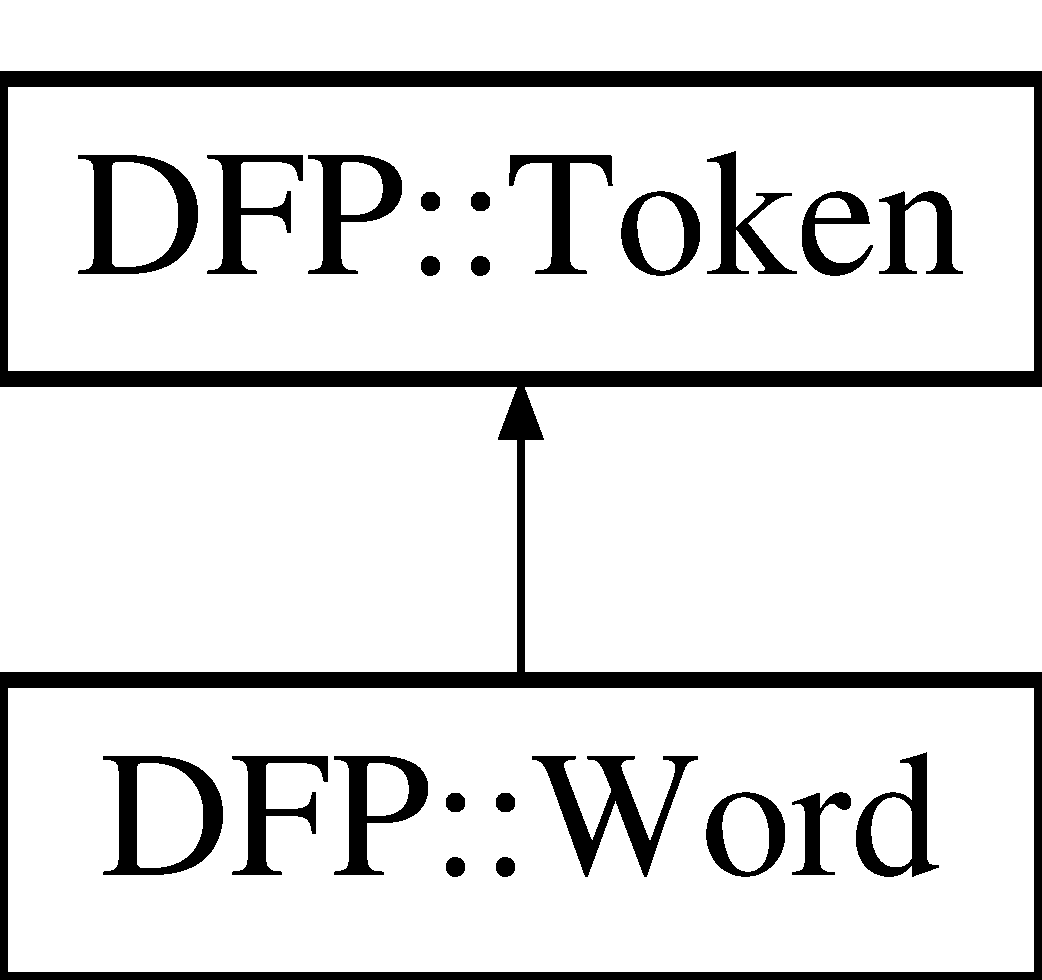
\includegraphics[height=2.000000cm]{class_d_f_p_1_1_word}
\end{center}
\end{figure}
\subsection*{Public Member Functions}
\begin{DoxyCompactItemize}
\item 
{\bfseries Word} (const char $\ast$v, int t)\hypertarget{class_d_f_p_1_1_word_af3baaa310a3edc2e98548364b94b216f}{}\label{class_d_f_p_1_1_word_af3baaa310a3edc2e98548364b94b216f}

\end{DoxyCompactItemize}
\subsection*{Public Attributes}
\begin{DoxyCompactItemize}
\item 
string\+\_\+t {\bfseries lexeme}\hypertarget{class_d_f_p_1_1_word_aba4633664b6a91b0d2ca6e4f0e2f23f2}{}\label{class_d_f_p_1_1_word_aba4633664b6a91b0d2ca6e4f0e2f23f2}

\end{DoxyCompactItemize}
\subsection*{Static Public Attributes}
\begin{DoxyCompactItemize}
\item 
static \hyperlink{class_d_f_p_1_1_word}{Word} $\ast$ {\bfseries ls} = new \hyperlink{class_d_f_p_1_1_word}{Word}(\char`\"{}\mbox{[}\char`\"{}, L\+S\+Q\+U\+A\+RE)\hypertarget{class_d_f_p_1_1_word_a051ffa7f53cc439afc32f542ac16f5ca}{}\label{class_d_f_p_1_1_word_a051ffa7f53cc439afc32f542ac16f5ca}

\item 
static \hyperlink{class_d_f_p_1_1_word}{Word} $\ast$ {\bfseries rs} = new \hyperlink{class_d_f_p_1_1_word}{Word}(\char`\"{}\mbox{]}\char`\"{}, R\+S\+Q\+U\+A\+RE)\hypertarget{class_d_f_p_1_1_word_aa1666db4d244aec9a7ec3f6ee4d3ba73}{}\label{class_d_f_p_1_1_word_aa1666db4d244aec9a7ec3f6ee4d3ba73}

\item 
static \hyperlink{class_d_f_p_1_1_word}{Word} $\ast$ {\bfseries lc} = new \hyperlink{class_d_f_p_1_1_word}{Word}(\char`\"{}\{\char`\"{}, L\+C\+U\+R\+LY)\hypertarget{class_d_f_p_1_1_word_ab43a22bed9227918e47158aa37074d04}{}\label{class_d_f_p_1_1_word_ab43a22bed9227918e47158aa37074d04}

\item 
static \hyperlink{class_d_f_p_1_1_word}{Word} $\ast$ {\bfseries rc} = new \hyperlink{class_d_f_p_1_1_word}{Word}(\char`\"{}\}\char`\"{}, R\+C\+U\+R\+LY)\hypertarget{class_d_f_p_1_1_word_a420040354de30da67547d0d537d2c0e2}{}\label{class_d_f_p_1_1_word_a420040354de30da67547d0d537d2c0e2}

\item 
static \hyperlink{class_d_f_p_1_1_word}{Word} $\ast$ {\bfseries arrow} = new \hyperlink{class_d_f_p_1_1_word}{Word}(\char`\"{}-\/$>$\char`\"{}, A\+R\+R\+OW)\hypertarget{class_d_f_p_1_1_word_aa6e71e3441f967b6b833d2206ae4324c}{}\label{class_d_f_p_1_1_word_aa6e71e3441f967b6b833d2206ae4324c}

\item 
static \hyperlink{class_d_f_p_1_1_word}{Word} $\ast$ {\bfseries colon} = new \hyperlink{class_d_f_p_1_1_word}{Word}(\char`\"{};\char`\"{}, C\+O\+L\+ON)\hypertarget{class_d_f_p_1_1_word_aa2a31e532e97b963ef604b425f36e456}{}\label{class_d_f_p_1_1_word_aa2a31e532e97b963ef604b425f36e456}

\end{DoxyCompactItemize}


The documentation for this class was generated from the following files\+:\begin{DoxyCompactItemize}
\item 
include/dfp\+\_\+lexer.\+hh\item 
src/dfp\+\_\+lexer.\+cc\end{DoxyCompactItemize}

%--- End generated contents ---

% Index
\backmatter
\newpage
\phantomsection
\clearemptydoublepage
\addcontentsline{toc}{chapter}{Index}
\printindex

\end{document}
